%\documentclass[10pt, compress, handout]{beamer} % no animations
\documentclass[10pt, compress]{beamer}
\usetheme{m}

\usepackage{booktabs}
\usepackage[scale=2]{ccicons}
\usepackage{minted}
\usepackage{color}
\usepackage{subfig}
\usepackage{xltxtra}
\usepackage{xgreek}	
\usepackage{amsfonts}
\usepackage[Greek,Latin]{ucharclasses}
\setTransitionsForGreek{\setlanguage{greek}}{\setlanguage{american}}
\setmainfont[Kerning=On,Mapping=tex-text]{Linux Libertine O}
\usepackage{amsmath}
\usepackage{amssymb}
\usepackage{outlines}
\usepackage[normalem]{ulem}
\usepackage{url}
\usepackage{tabularx}
\usepackage{graphicx}

\usepackage{placeins}

\usepackage{multirow}

\usemintedstyle{trac}

\usepackage[backend=biber, sorting=none, maxcitenames=2]{biblatex}
\addbibresource{references.bib} % The filename of the bibliography

\title{Ανάπτυξη Αυτόνομου Ρομποτικού Οχήματος Εδάφους με Κινηματικό Μοντέλο 4WS4WD και Υλοποίηση Συστήματος για Αυτόνομη Εξερεύνηση σε Άγνωστο Περιβάλλον}
\date{4 Νοεμβρίου, 2016}
\author{Γεώργιος Κούρος}
\institute{Αριστοτέλειο Πανεπιστήμιο Θεσσαλονίκης\\[-0.1cm]Τμήμα Ηλεκτρολόγων Μηχανικών και Μηχανικών Υπολογιστών\\[-0.1cm]Τομέας Ηλεκτρονικής και Υπολογιστών}


\begin{document}

\maketitle

%%%%%%%%%%%%%%%%%%%%%%%%%%%%%%%%%%%%%%%%%%%%%%%%%%%%%%%%%%%%%%%%%%%%%%%%%%%%%%%%%%%%%%%%%%%%%%
\begin{frame}{Επισκόπηση}
	\begin{itemize}[<+- | alert@+>]
		\item{Κίνητρο}
		\item{Ρομποτική Πλατφόρμα Monstertruck}
		\item{Κινηματική Ανάλυση}
		\item{Εκτίμηση Κατάστασης και Χαρτογράφηση}
		\item{Αυτόνομη Πλοήγηση και Εξερεύνηση}
		\item{Εργαλεία και Αρχιτεκτονική Συστήματος}
		\item{Πειράματα}
		\item{Συμπεράσματα και Μελλοντική Εργασία}
	\end{itemize}
\end{frame}

%%%%%%%%%%%%%%%%%%%%%%%%%%%%%%%%%%%%%%%%%%%%%%%%%%%%%%%%%%%%%%%%%%%%%%%%%%%%%%%%%%%%%%%%%%%%%%
%%%%%%%%%%%%%%%%%%%%%%%%%%%%%%%%%%%%%%%%%%%%%%%%%%%%%%%%%%%%%%%%%%%%%%%%%%%%%%%%%%%%%%%%%%%%%%
\section{Κίνητρο}

%%%%%%%%%%%%%%%%%%%%%%%%%%%%%%%%%%%%%%%%%%%%%%%%%%%%%%%%%%%%%%%%%%%%%%%%%%%%%%%%%%%%%%%%%%%%%%
\begin{frame}{Κίνητρο}
	\visible<1-4>{
	\begin{figure}
		
\includegraphics[height=1.5cm]{Figures/pandora-logo.png}\\
	\end{figure}}
	\visible<2-4>{	
	\begin{figure}[!ht] \centering
		\begin{tikzpicture}
			\pause
		   \node (pandora_tracked_robot) {\frame{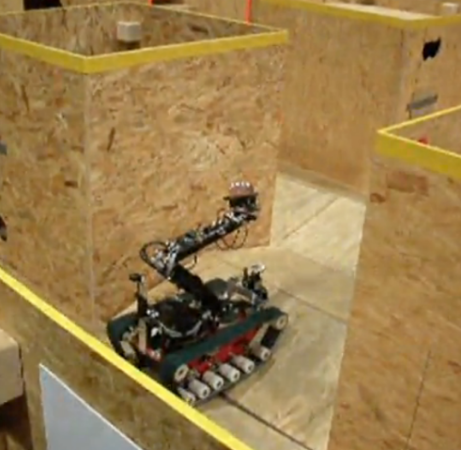
\includegraphics[height=3.5cm]{pandora_tracked_robot.png}}};
	   		\pause
   		   \node (pandora_skid_steer_robot) at (pandora_tracked_robot.south east) [yshift=1cm] [xshift=1cm] {\frame{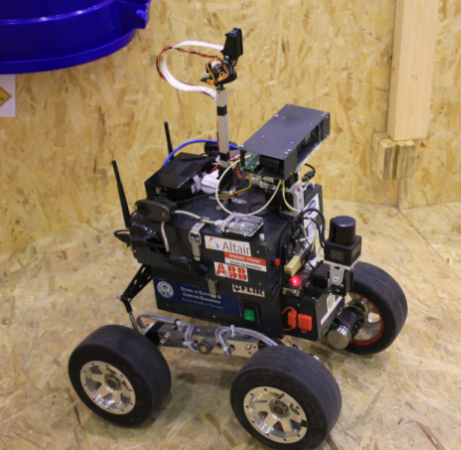
\includegraphics[height=3.5cm]{pandora_skid_steer_robot.png}}};
	   		\pause
		   	\node (pandora_monstertruck) at (pandora_skid_steer_robot.south east) [yshift=1cm][xshift=1cm] {\frame{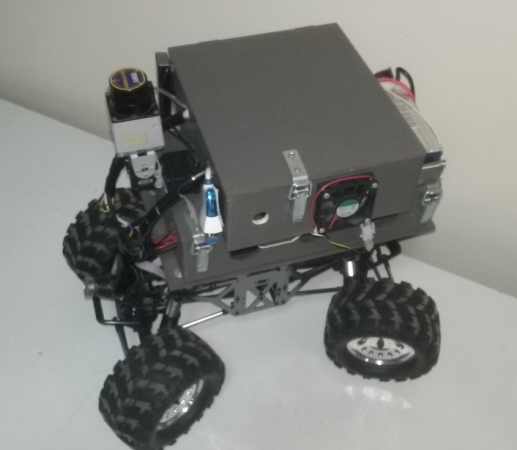
\includegraphics[height=3.5cm]{pandora_monstertruck.png}}};
		\end{tikzpicture}
	\end{figure}}
\end{frame}

%%%%%%%%%%%%%%%%%%%%%%%%%%%%%%%%%%%%%%%%%%%%%%%%%%%%%%%%%%%%%%%%%%%%%%%%%%%%%%%%%%%%%%%%%%%%%%
%%%%%%%%%%%%%%%%%%%%%%%%%%%%%%%%%%%%%%%%%%%%%%%%%%%%%%%%%%%%%%%%%%%%%%%%%%%%%%%%%%%%%%%%%%%%%%
\section{Ρομποτική Πλατφόρμα Monstertruck}

%%%%%%%%%%%%%%%%%%%%%%%%%%%%%%%%%%%%%%%%%%%%%%%%%%%%%%%%%%%%%%%%%%%%%%%%%%%%%%%%%%%%%%%%%%%%%%
\begin{frame}{Βάση}
	Τηλεκατευθυνόμενο Όχημα \textbf{Groundpounder}, της Redcat Racing.\\[1cm]
	
	\begin{minipage}{0.55\textwidth}
		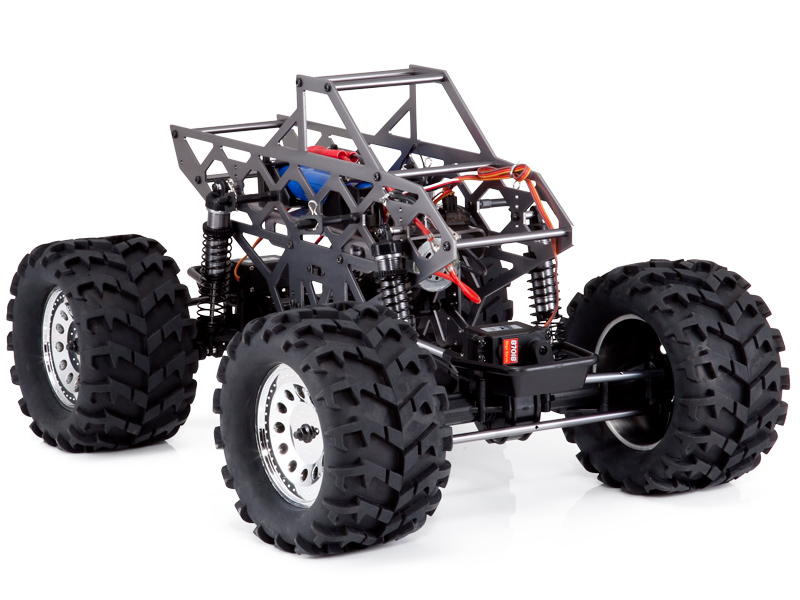
\includegraphics[width=\textwidth]{Figures/groundpounder.jpg}
	\end{minipage}
	\begin{minipage}{0.4\textwidth}
		\begin{itemize}
			\item Τετρακίνηση - 4WD
			\item Τετραδιεύθυνση - 4WS
			\item Κλίμακα 1:10
			\item Αναρτήσεις
			\item Μεταλλικό Σασί
			\item Τροχοί Offroad
		\end{itemize}
	\end{minipage}
	
\end{frame}

%%%%%%%%%%%%%%%%%%%%%%%%%%%%%%%%%%%%%%%%%%%%%%%%%%%%%%%%%%%%%%%%%%%%%%%%%%%%%%%%%%%%%%%%%%%%%%
\begin{frame}{Εξοπλισμός}
	\begin{figure}
		\visible<1-3>{\subfloat{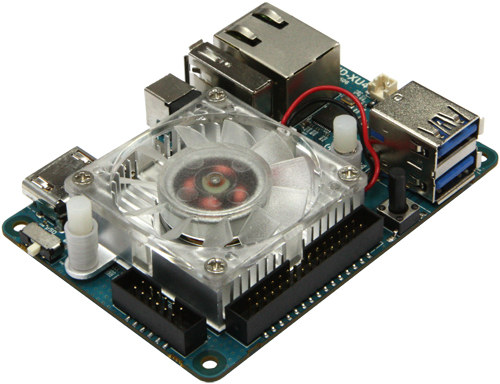
\includegraphics[height=3.5cm]{Figures/odroid-xu4.jpg}}}\\
		\visible<2-3>{\subfloat{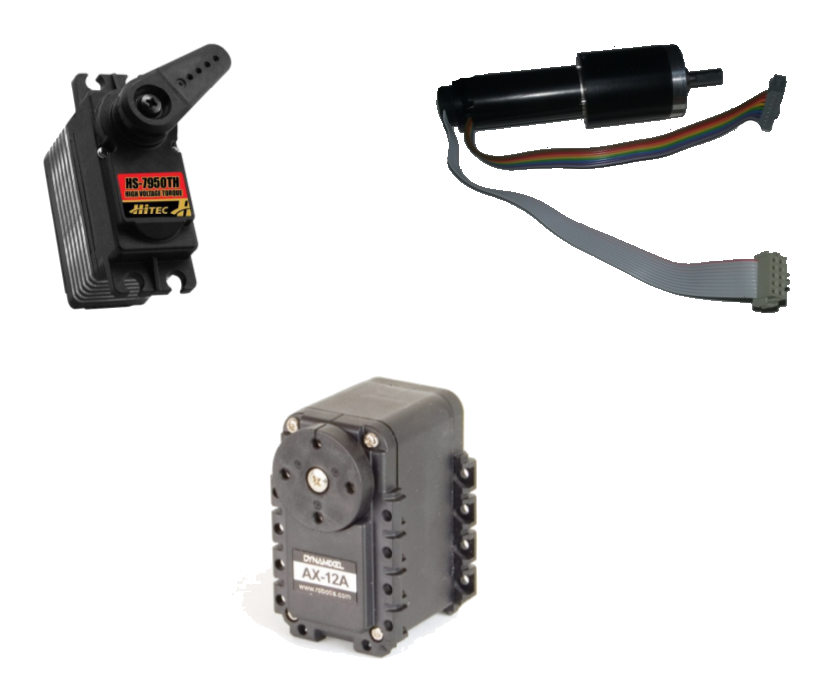
\includegraphics[width=0.45\linewidth]{Figures/motors.png}}}
		\hspace{0.03\linewidth}
		\visible<3>{\subfloat{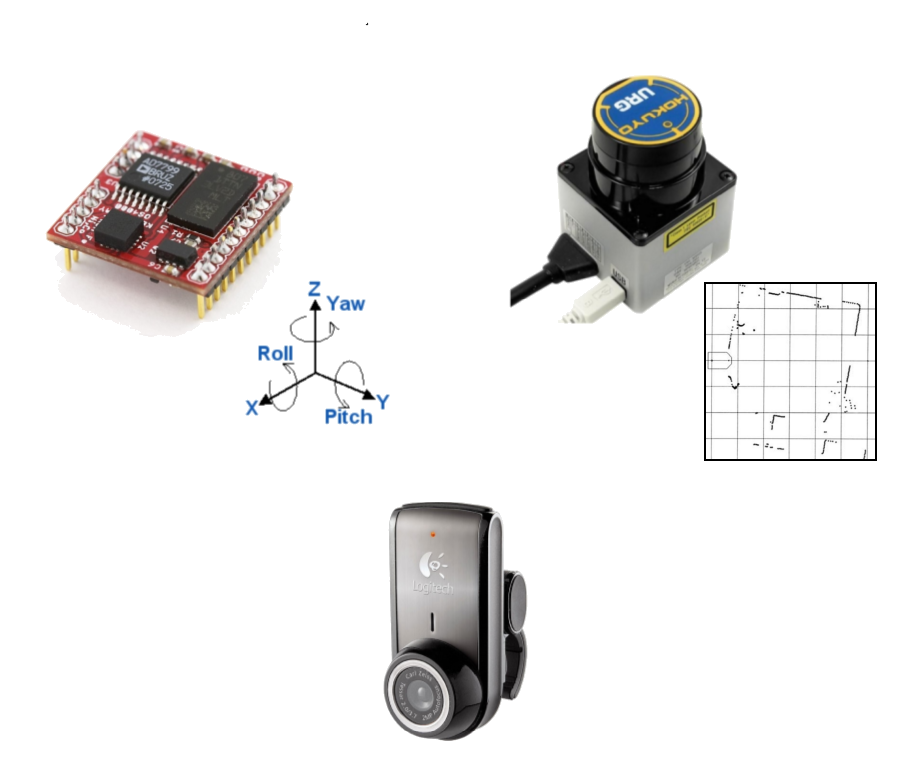
\includegraphics[width=0.45\linewidth]{Figures/sensors.png}}}
	\end{figure}
\end{frame}

%%%%%%%%%%%%%%%%%%%%%%%%%%%%%%%%%%%%%%%%%%%%%%%%%%%%%%%%%%%%%%%%%%%%%%%%%%%%%%%%%%%%%%%%%%%%%%
%%%%%%%%%%%%%%%%%%%%%%%%%%%%%%%%%%%%%%%%%%%%%%%%%%%%%%%%%%%%%%%%%%%%%%%%%%%%%%%%%%%%%%%%%%%%%%
\section{Κινηματική Ανάλυση}

%%%%%%%%%%%%%%%%%%%%%%%%%%%%%%%%%%%%%%%%%%%%%%%%%%%%%%%%%%%%%%%%%%%%%%%%%%%%%%%%%%%%%%%%%%%%%%
\begin{frame}{Σύστημα Μετάδοσης Κίνησης}
%	\begin{equation*}
%		\omega_{wheel} = \omega_{motor} / (\lambda_{gearbox} \times \lambda_{spur\_pinion} \times \lambda_{transfer\_case} \times \lambda_{differential}) = \omega_{motor} / 644
%	\end{equation*}
	\begin{minipage}{0.7\linewidth}
		\begin{figure}
			\subfloat{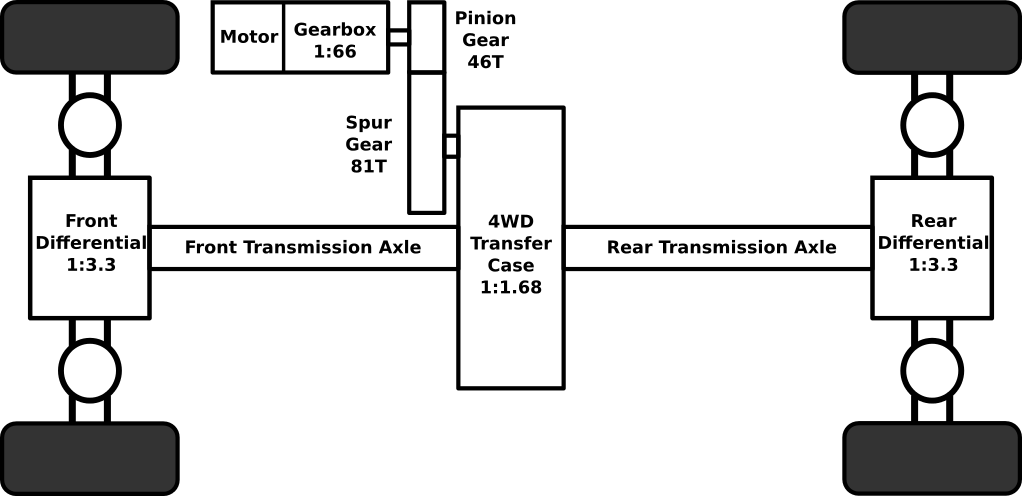
\includegraphics[width=\textwidth]{Figures/drivetrain.png}}\\
			\subfloat{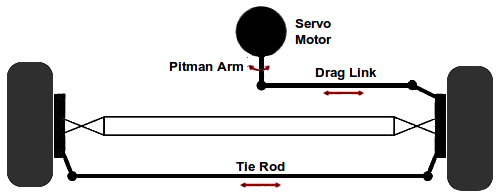
\includegraphics[width=\textwidth]{Figures/my_drag_link_steering.png}}
		\end{figure}
	\end{minipage}%
	\begin{minipage}{0.3\linewidth}
		\begin{figure}
			\centering
			\subfloat{\frame{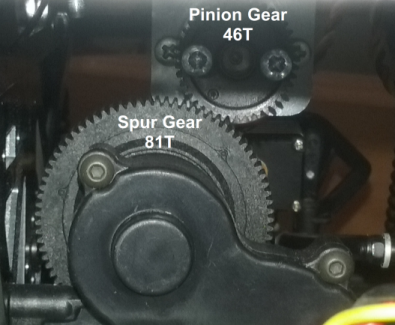
\includegraphics[width=2.25cm]{Figures/spur_and_pinion_gears.png}}}\\[0.1cm]
			\subfloat{\frame{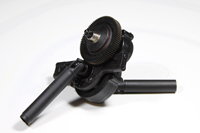
\includegraphics[width=2.25cm]{Figures/transfer_case.jpg}}}\\[0.1cm]
			\subfloat{\frame{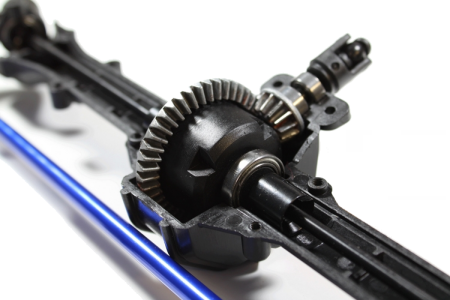
\includegraphics[width=2.25cm]{Figures/differential.png}}}\\[0.1cm]
			\subfloat{\frame{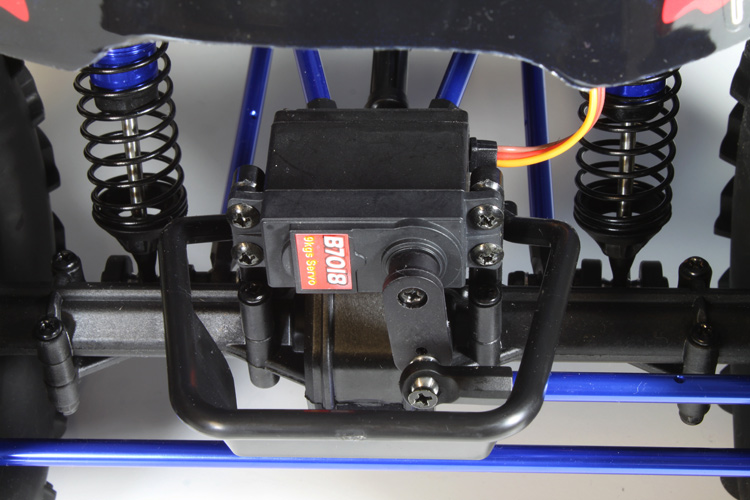
\includegraphics[width=2.25cm]{Figures/drag_link_real.jpg}}}
		\end{figure}
	\end{minipage}
\end{frame}

%%%%%%%%%%%%%%%%%%%%%%%%%%%%%%%%%%%%%%%%%%%%%%%%%%%%%%%%%%%%%%%%%%%%%%%%%%%%%%%%%%%%%%%%%%%%%%
%\begin{frame}{Σύστημα Τετραδιεύθυνσης}
%	\begin{figure}
%		\centering
%		\visible<1-4>{
%		\subfloat{{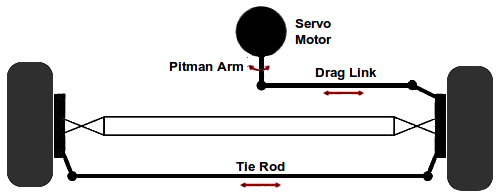
\includegraphics[width=0.5\linewidth]{Figures/my_drag_link_steering.png}}}} \\[0.15cm]
%		\visible<2-4>{		
%		\subfloat{{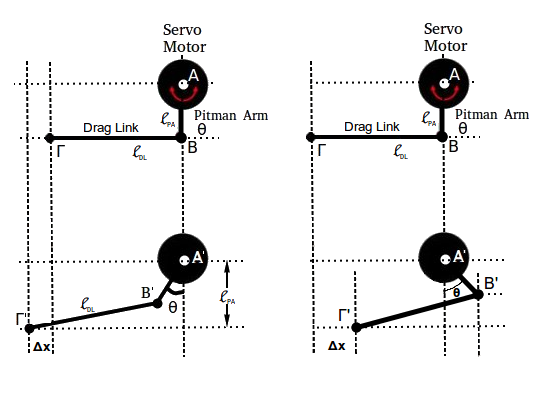
\includegraphics[height=4cm]{Figures/drag_link_analysis.png}}}}
%		\hspace{0.5cm}
%		\visible<3-4>{
%		\subfloat{{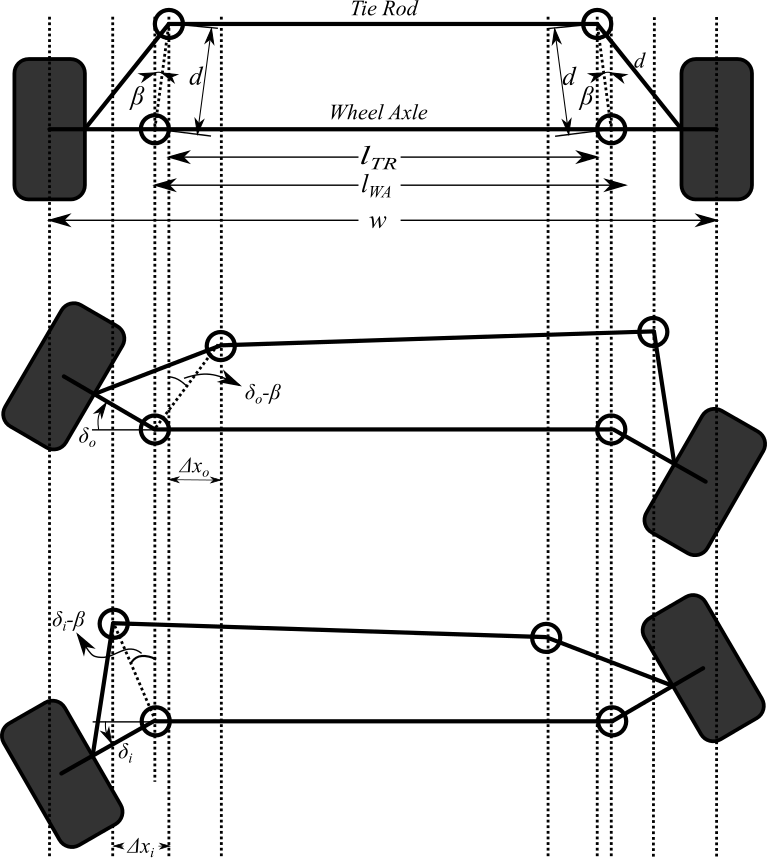
\includegraphics[height=4cm]{Figures/trapezoid_steering_mechanism}}}} \\[0.05cm]
%		\visible<4>{
%		\subfloat{{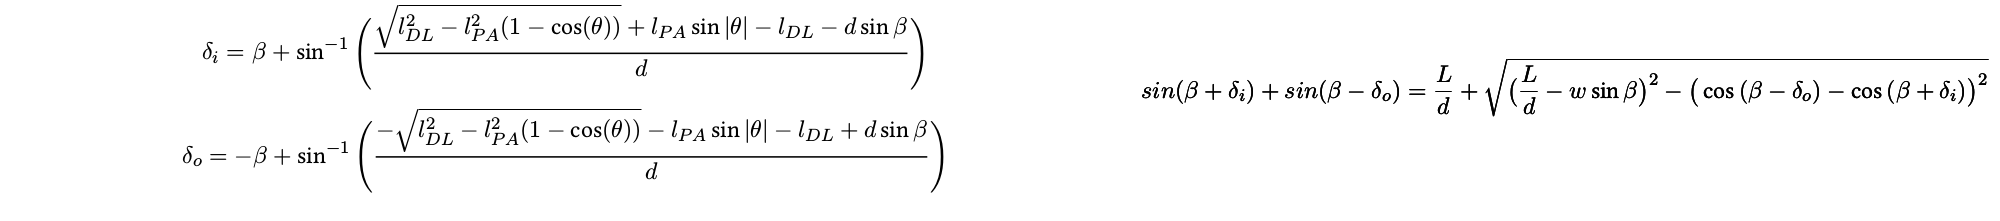
\includegraphics[width=\linewidth]{Figures/steering_transfer.png}}}}
%	\end{figure}
%\end{frame}

%%%%%%%%%%%%%%%%%%%%%%%%%%%%%%%%%%%%%%%%%%%%%%%%%%%%%%%%%%%%%%%%%%%%%%%%%%%%%%%%%%%%%%%%%%%%%%
%\begin{frame}{Κινηματικό Μοντέλο Ackermann}
%	\begin{figure}
%		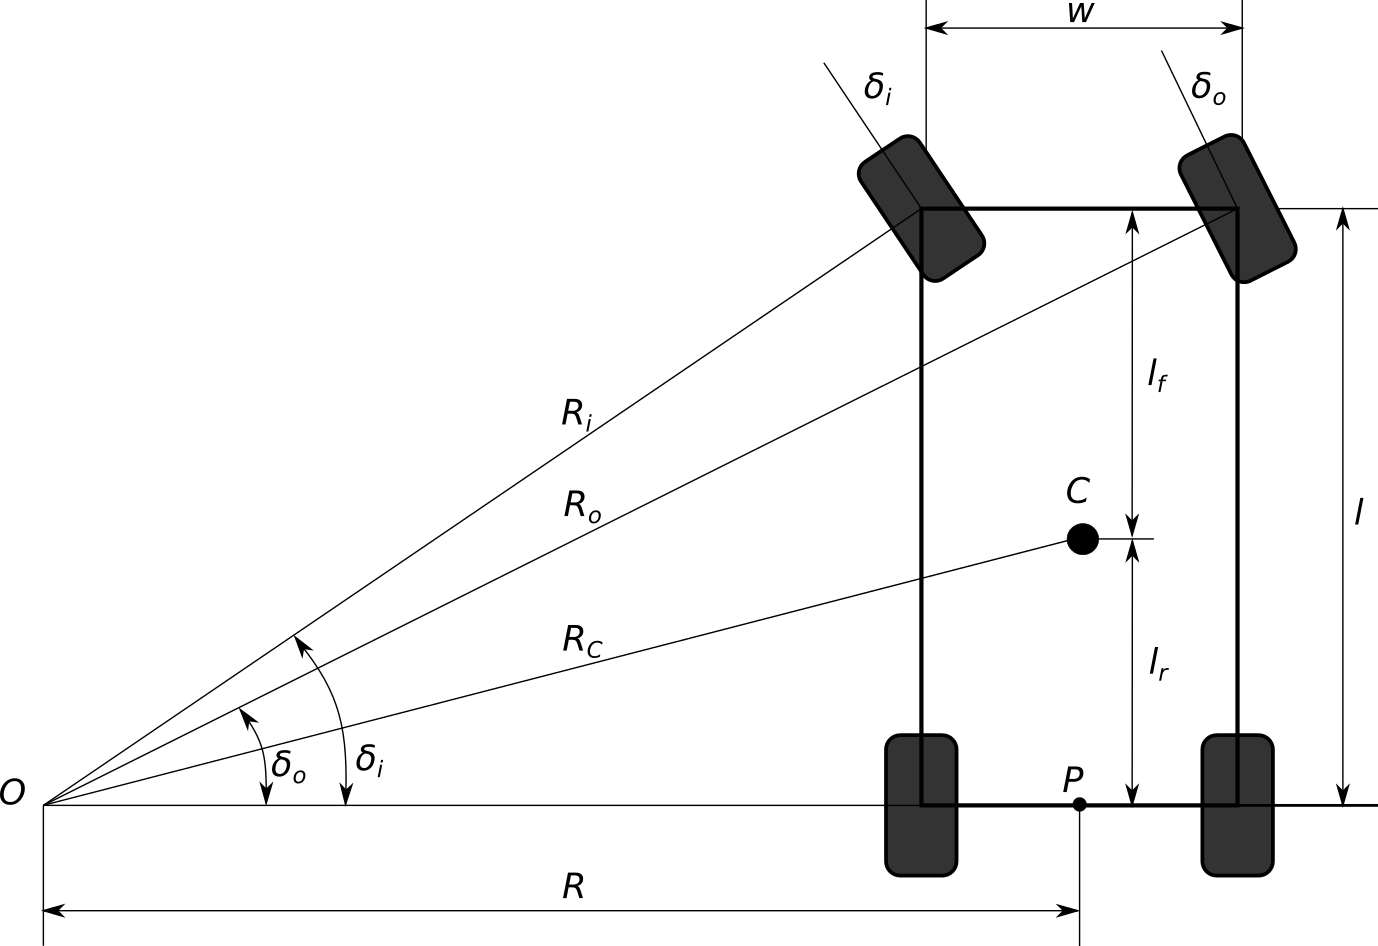
\includegraphics[height=5cm]{Figures/ackermann_model.png}
%	\end{figure}
%	\visible<2>{
%	\textbf{Συνθήκη Ackermann: }
%	\begin{equation*}
%		\cot{\delta_i} - \cot{\delta_o} = w / l
%	\end{equation*}}
%\end{frame}

%%%%%%%%%%%%%%%%%%%%%%%%%%%%%%%%%%%%%%%%%%%%%%%%%%%%%%%%%%%%%%%%%%%%%%%%%%%%%%%%%%%%%%%%%%%%%%
\begin{frame}{Κινηματικό Μοντέλο Τετραδιεύθυνσης (4WS)}
	\begin{figure}[!ht]
		\visible<1-3>{\subfloat{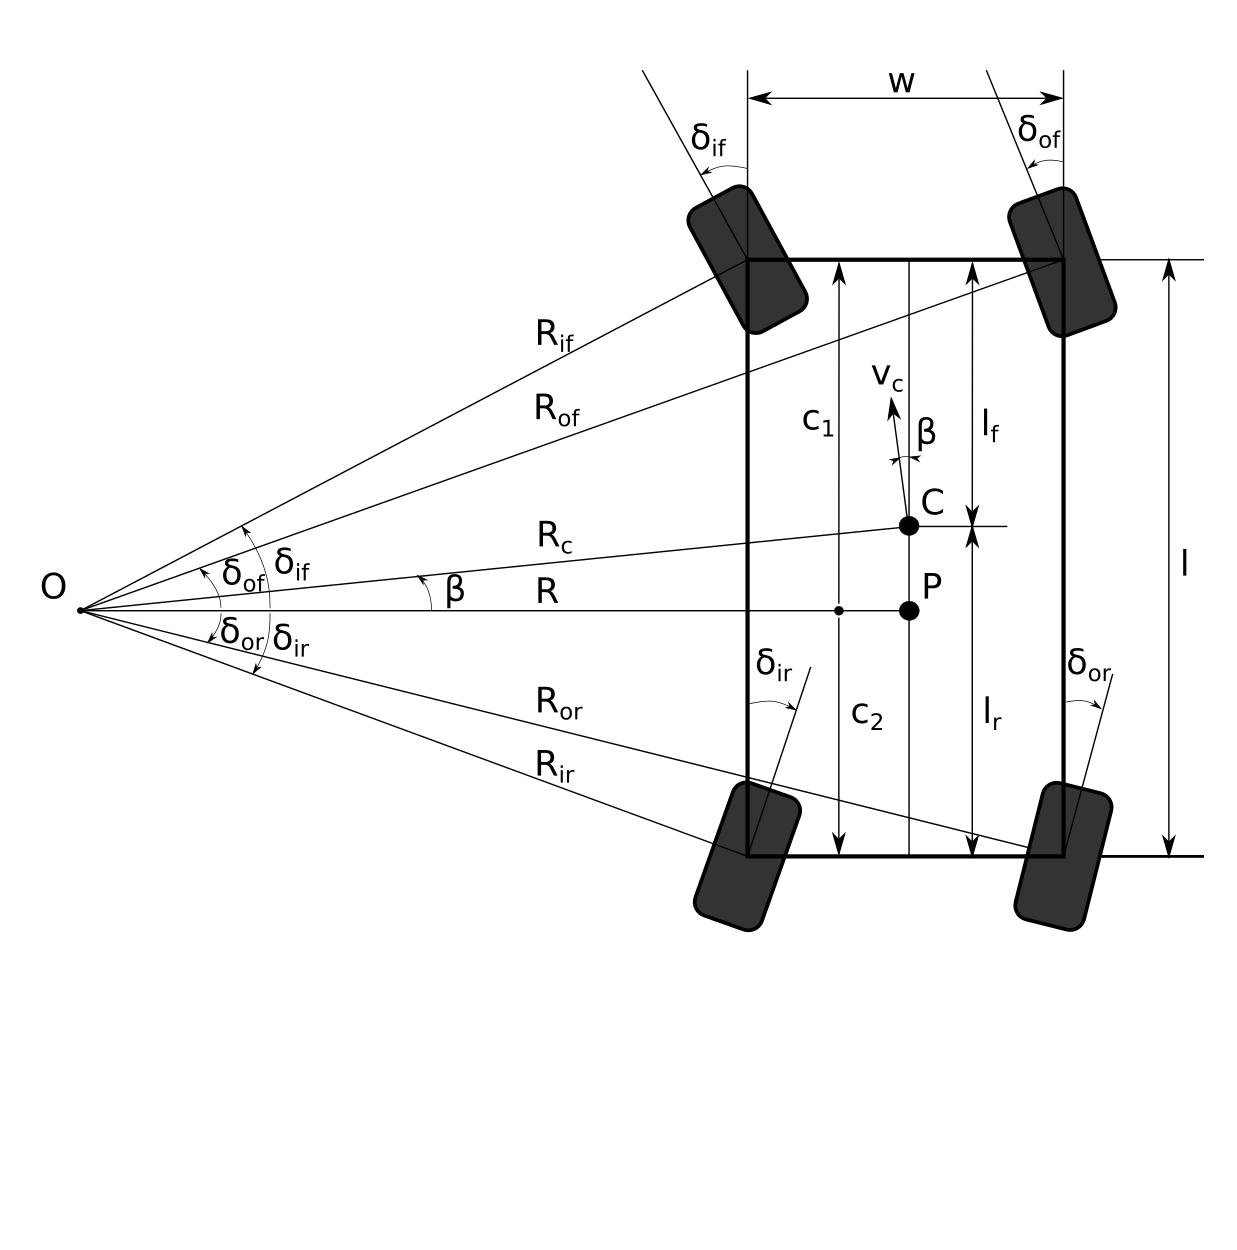
\includegraphics[height=5.2cm]{Figures/4ws_model.png}}}
		\visible<2-3>{\subfloat{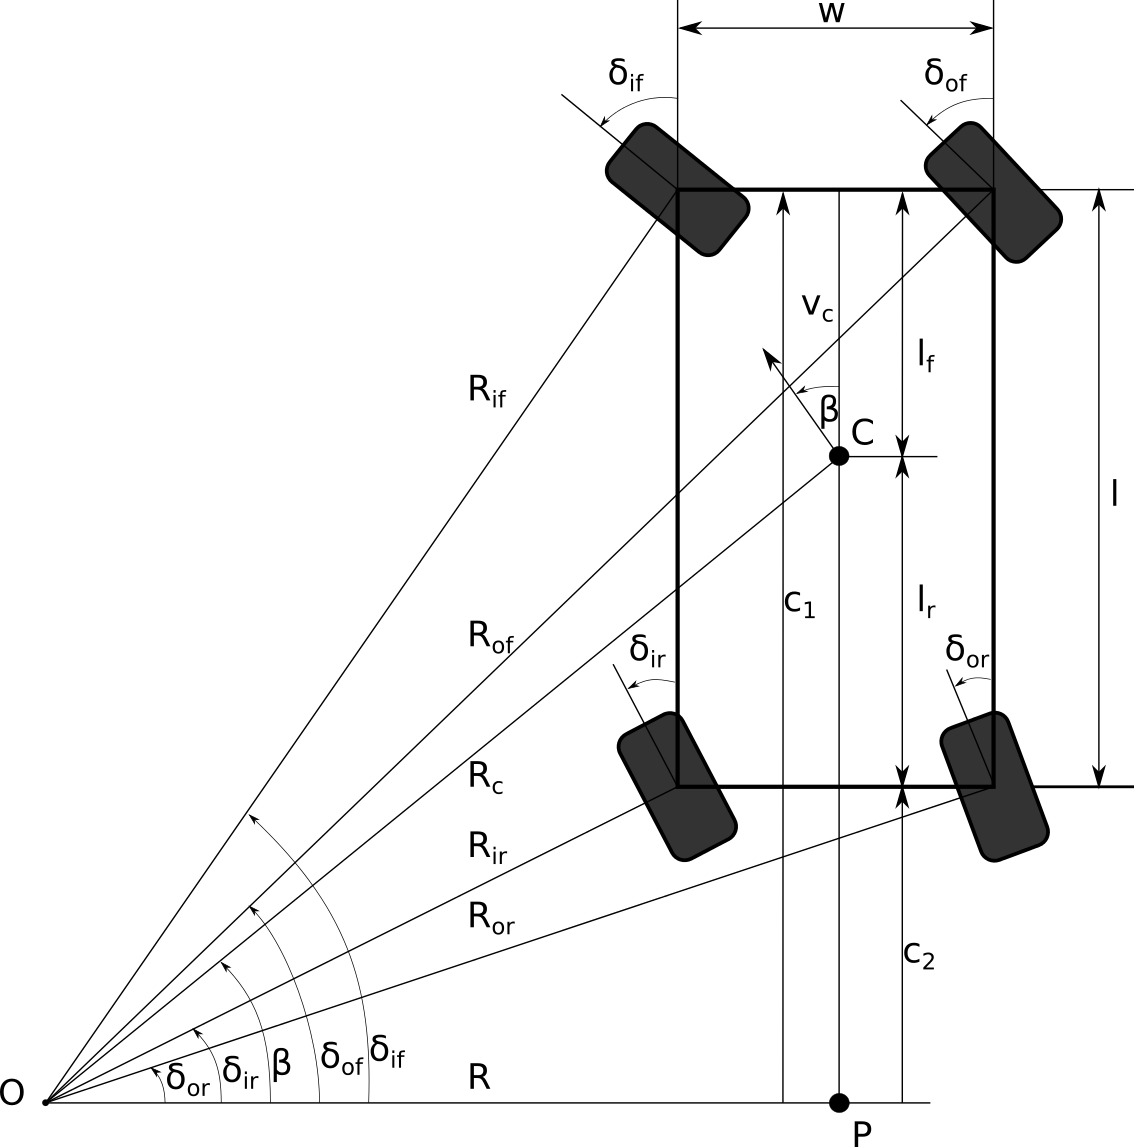
\includegraphics[height=5cm]{Figures/pos_4ws_model.png}}}
	\end{figure}
	\visible<3>{	
	\textbf{Συνθήκη Τετραδιεύθυνσης:}
	\begin{equation*}
		\frac{1}{\cot{\delta_{of}} - \cot{\delta_{if}}} + \frac{1}{\cot{\delta_{or}} - 	\cot{\delta_{ir}}} = \frac{l}{w}
	\end{equation*}}
\end{frame}

%%%%%%%%%%%%%%%%%%%%%%%%%%%%%%%%%%%%%%%%%%%%%%%%%%%%%%%%%%%%%%%%%%%%%%%%%%%%%%%%%%%%%%%%%%%%%%
\begin{frame}{Κινηματικό Μοντέλο Ρομποτικής Πλατφόρμας Monstertruck}
	\begin{figure}
		\subfloat{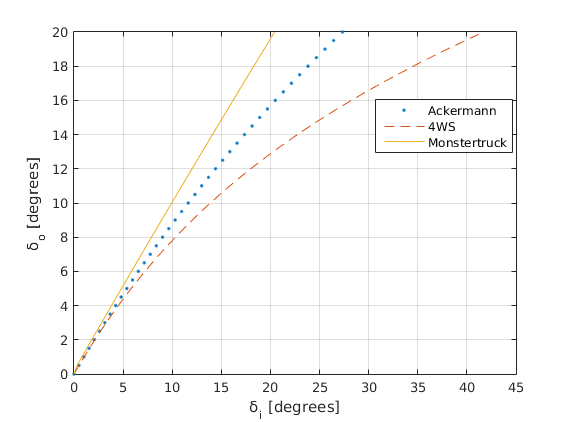
\includegraphics[height=3.0cm]{Figures/steer_angles_comparison.png}}
%		\hspace{1cm}
		\subfloat{\includegraphics<1>[height=3.5cm]{Figures/monstertruck_model_parallel.png}}
		\subfloat{\includegraphics<2-3>[height=3.5cm]{Figures/monstertruck_slip_angle_model_parallel.png}}\\
		\subfloat{\includegraphics<2-3>[height=2.0cm]{Figures/monstertruck_slip_angles.png}}
	\end{figure}
	\visible<3>{
	\textbf{Μη Ιδανική Συνθήκη Τετραδιεύθυνσης:}
	\begin{equation*}
		\frac{1}{\cot(\delta_{of} - \alpha_{of}) - \cot(\delta_{if} + \alpha_{if})} - \frac{1}{\cot(\delta_{or} - \alpha_{or}) - \cot(\delta_{ir} + \alpha_{ir})} = \frac{l}{w}
	\end{equation*}}
	\vspace{3cm}
\end{frame}


%%%%%%%%%%%%%%%%%%%%%%%%%%%%%%%%%%%%%%%%%%%%%%%%%%%%%%%%%%%%%%%%%%%%%%%%%%%%%%%%%%%%%%%%%%%%%%
%%%%%%%%%%%%%%%%%%%%%%%%%%%%%%%%%%%%%%%%%%%%%%%%%%%%%%%%%%%%%%%%%%%%%%%%%%%%%%%%%%%%%%%%%%%%%%
\section{Εκτίμηση Κατάστασης και Χαρτογράφηση}

%%%%%%%%%%%%%%%%%%%%%%%%%%%%%%%%%%%%%%%%%%%%%%%%%%%%%%%%%%%%%%%%%%%%%%%%%%%%%%%%%%%%%%%%%%%%%%
%\begin{frame}{Κατάσταση και SLAM}
%	\begin{itemize}
%		\item Κατάσταση:  $s_{6D}=(x,y,z,\phi,\psi,\theta)\; \text{ή}\; (x,y,z,roll,pitch,yaw)$
%		\item 2D Χαρτογράφηση $\rightarrow$ 3D κατάσταση $\rightarrow$ πόζα $p=(x,y,\theta)$
%    	\item	\textbf{SLAM}: \textbf{S}imultaneous \textbf{L}ocalization \textbf{A}nd \textbf{M}apping
%		\item Χάρτες Πλέγματος Κατάληψης (OGM)
%		\item Αξιοποίηση πληροφορίας από σαρωτές λέιζερ
%	\end{itemize}
%	\vspace{-0.5cm}
%	\begin{figure}[!ht]
%		\subfloat{\frame{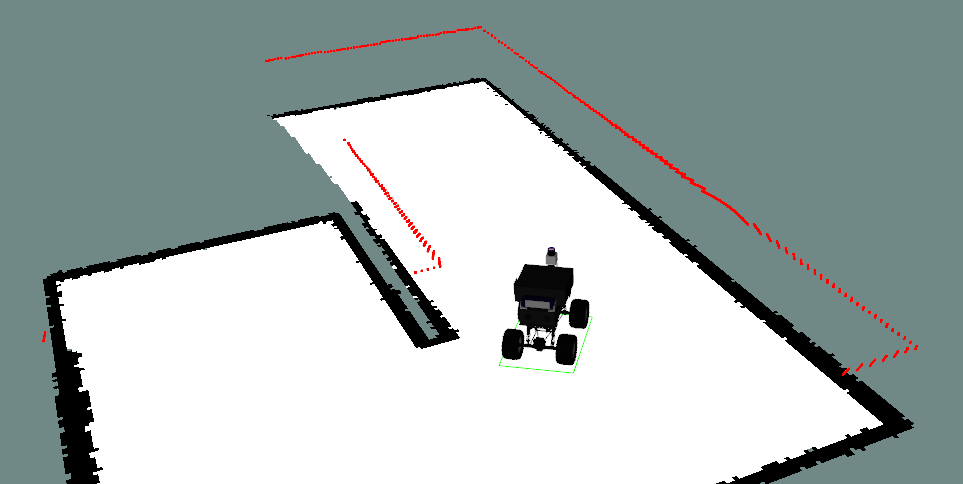
\includegraphics[height=3.3cm]{Figures/map_and_scan.png}}}
%		\hspace{0.1cm}
%		\subfloat{\frame{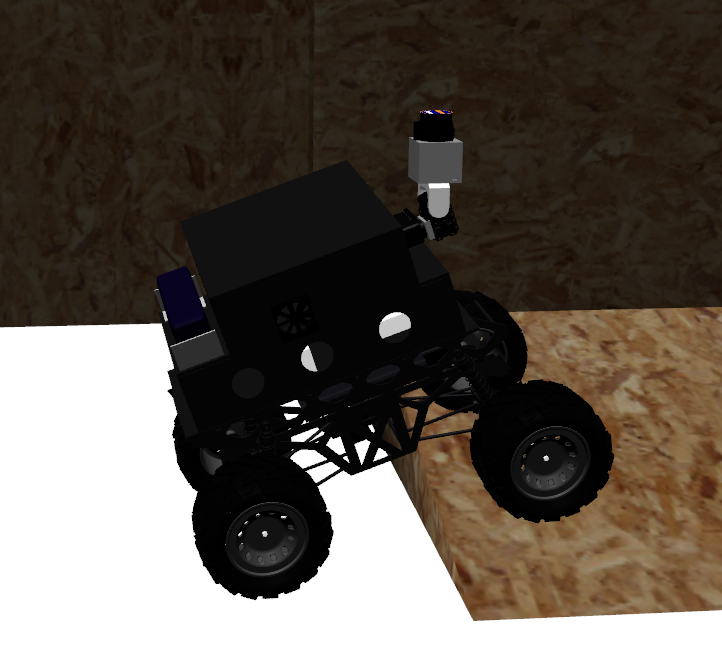
\includegraphics[height=3.3cm]{Figures/stabilized_laser.png}}}
%	\end{figure}		
%\end{frame}

%%%%%%%%%%%%%%%%%%%%%%%%%%%%%%%%%%%%%%%%%%%%%%%%%%%%%%%%%%%%%%%%%%%%%%%%%%%%%%%%%%%%%%%%%%%%%%
\begin{frame}{SLAM}
	\begin{itemize}
		\item \textbf{SLAM}: \textbf{S}imultaneous \textbf{L}ocalization \textbf{A}nd \textbf{M}apping\\
		\item 2D Χαρτογράφηση $\rightarrow$ Occupancy Grid Maps
		\item Εντοπισμός πόζας $p=(x,y,\theta)$
	\end{itemize}		
	\vspace{-0.5cm}
	\begin{figure}[!ht]
		\subfloat{\frame{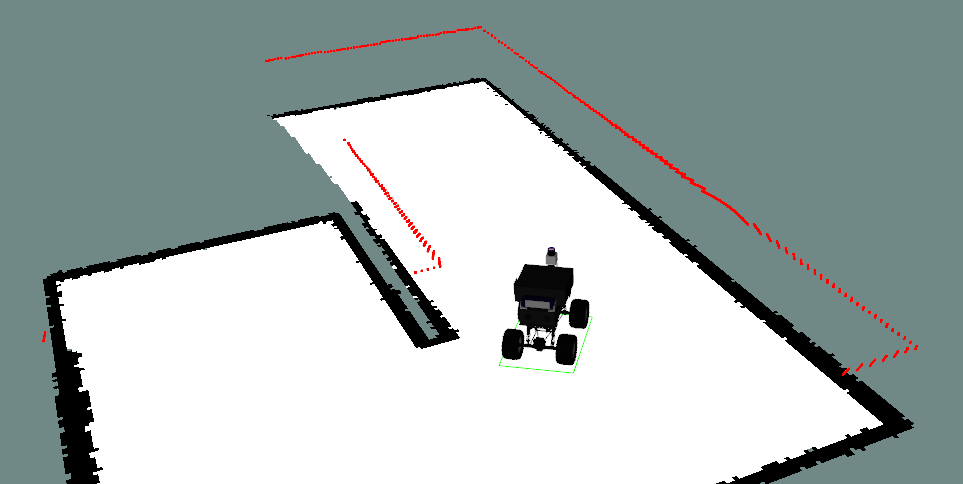
\includegraphics[height=3cm]{Figures/map_and_scan.png}}}
		\hspace{1cm}
		\subfloat{\frame{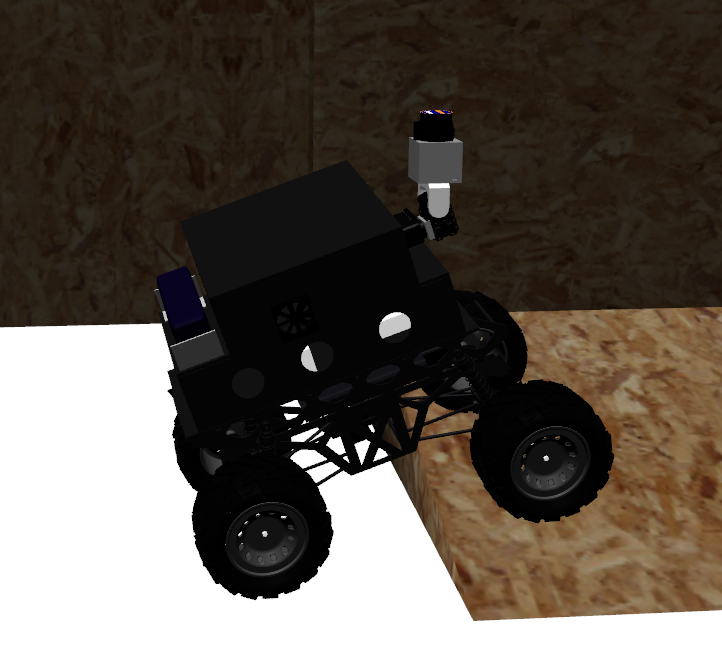
\includegraphics[height=3cm]{Figures/stabilized_laser.png}}}
	\end{figure}
	\vspace{-0.3cm}
	\begin{minipage}[t]{0.55\textwidth}
		\visible<2-3>{
		\textbf{CRSM-SLAM}
		\begin{itemize}
			\item \textbf{C}ritical \textbf{R}ays \textbf{S}can \textbf{M}atch
			\item Αντιστοίχιση σκαναρισμάτων\\$\rightarrow$ RRHC
			\item Προεπεξεργασία σκαναρισμάτων\\$\rightarrow$ επιλογή κρίσιμων ακτίνων
		\end{itemize}}	
	\end{minipage}%
	\begin{minipage}[t]{0.45\textwidth}
		\visible<3>{
		\textbf{Gmapping}
		\begin{outline}
			\1 Φίλτρα σωματιδίων
			\1 Εκτίμηση χάρτη και τροχιάς ρομπότ βάσει
				\2 σκαναρισμάτων
				\2 οδομετρίας			
		\end{outline}}
	\end{minipage}\\
\end{frame}

%%%%%%%%%%%%%%%%%%%%%%%%%%%%%%%%%%%%%%%%%%%%%%%%%%%%%%%%%%%%%%%%%%%%%%%%%%%%%%%%%%%%%%%%%%%%%%
%%%%%%%%%%%%%%%%%%%%%%%%%%%%%%%%%%%%%%%%%%%%%%%%%%%%%%%%%%%%%%%%%%%%%%%%%%%%%%%%%%%%%%%%%%%%%%
\section{Αυτόνομη Πλοήγηση και Εξερεύνηση}

%%%%%%%%%%%%%%%%%%%%%%%%%%%%%%%%%%%%%%%%%%%%%%%%%%%%%%%%%%%%%%%%%%%%%%%%%%%%%%%%%%%%%%%%%%%%%%
%\begin{frame}{Αυτόνομη Πλοήγηση}
%	\begin{itemize}
%		\item Στόχος: $\;\;p_{init}$ $\rightarrow$ $p_{final}$
%		\item Διάσπαση προβλήματος $\rightarrow$ ολικό και τοπικό
%		\item	Αναζήτηση λύσης σε χάρτες κόστους (costmaps)
%	\end{itemize}
%	\vspace{-0.5cm}
%	\begin{figure}
%		\centering
%		\subfloat{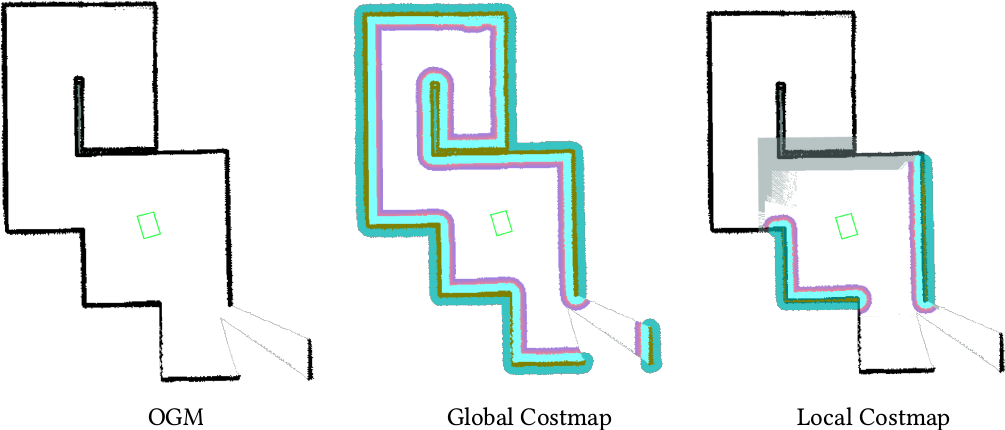
\includegraphics[width=0.8\linewidth]{Figures/costmaps.png}}
%	\end{figure}
%\end{frame}

%%%%%%%%%%%%%%%%%%%%%%%%%%%%%%%%%%%%%%%%%%%%%%%%%%%%%%%%%%%%%%%%%%%%%%%%%%%%%%%%%%%%%%%%%%%%%%
\begin{frame}{Προτάσεις}
	\begin{enumerate}
		\visible<1-2>{\item Αυτόνομη Πλοήγηση με Δυναμική Παραμόρφωση Μονοπατιού (DPM)
		\vspace{-0.5cm}
		\begin{enumerate}
			\item Κατασκευή στατικού ολικού μονοπατιού $\rightarrow$ Dijkstra / A*
			\item Μετατροπή ολικού μονοπατιού σε τοπικό $\rightarrow$ Reeds-Shepp Band
			\item Διάσχιση τοπικού μονοπατιού $\rightarrow$ ελεγκτής ασαφούς λογικής
		\end{enumerate}}
		
		\visible<2>{\item Αυτόνομη Πλοήγηση με Δυναμική Ανακατασκευή Μονοπατιού (DPR)
		\begin{enumerate}
			\item Δυναμική ανακατασκευή ολικού μονοπατιού $\rightarrow$ SBPL Lattice Planner
			\item Διάσχιση ολικού μονοπατιού $\rightarrow$ ελεγκτής ασαφούς λογικής
		\end{enumerate}}
		
	\end{enumerate}
	\begin{figure}
		\centering
		\visible<1-2>{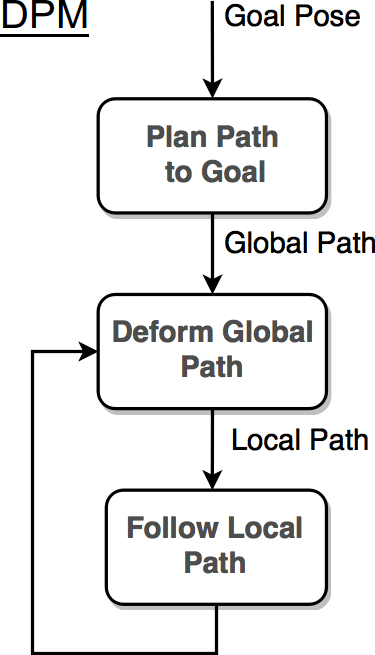
\includegraphics[width=2cm]{Figures/dpm.png}}
		\hspace{2cm}
		\visible<2>{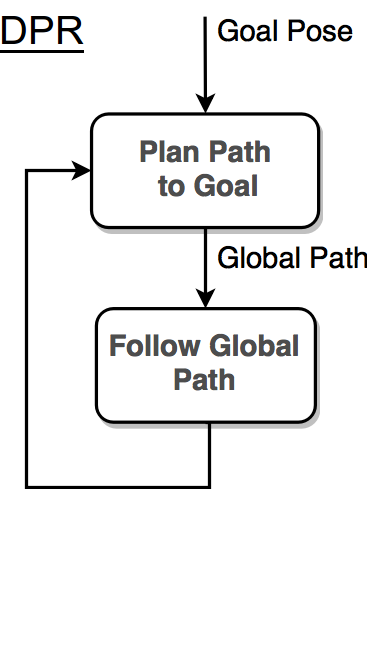
\includegraphics[width=2cm]{Figures/dpr.png}}
	\end{figure}
\end{frame}

%%%%%%%%%%%%%%%%%%%%%%%%%%%%%%%%%%%%%%%%%%%%%%%%%%%%%%%%%%%%%%%%%%%%%%%%%%%%%%%%%%%%%%%%%%%%%%
\begin{frame}{DPM (1/3): Ολικό Μονοπάτι μέσω Dijkstra ή Α*}
	\begin{itemize}
		\item Κατασκευή ολικού μονοπατιού $\rightarrow$ graph-search
		\item Dijkstra $\rightarrow$ Breadth-First Search $\rightarrow$ $f(n)=g(n)$
		\item Α* $\rightarrow$ μεταξύ Breadth-First, Best-First Search $\rightarrow$ $f(n)=g(n)+h(n)$
		\item Dijkstra $\rightarrow$ πάντα βέλτιστη λύση, αλλά Α* $\rightarrow$ αποδοτικότερος
		\item \underline{Κινηματικά μη εφικτό μονοπάτι} για Car-Like Robots
	\end{itemize}
	\vspace{-0.2cm}
	\begin{figure}
		\captionsetup[subfigure]{labelformat=empty}
		\subfloat[Dijkstra]{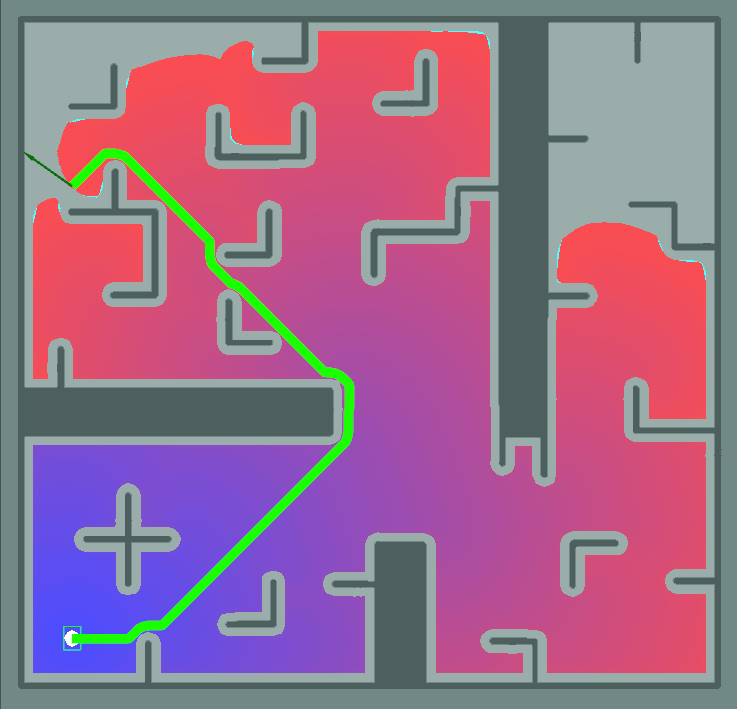
\includegraphics[width=0.4\linewidth]{Figures/so_dijkstra_p4.png}}
		\hspace{1cm}
		\subfloat[A*]{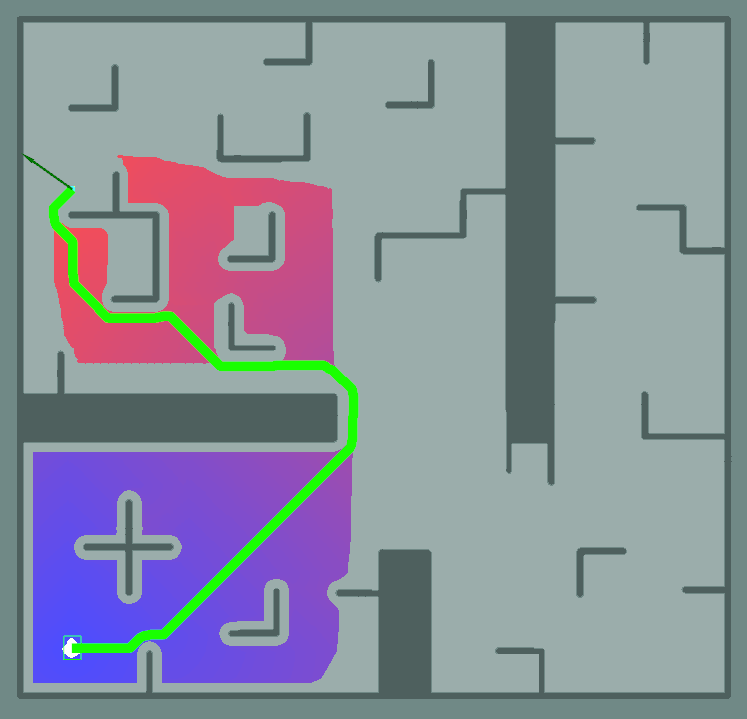
\includegraphics[width=0.4\linewidth]{Figures/so_astar_p4.png}}
	\end{figure}
\end{frame}

%%%%%%%%%%%%%%%%%%%%%%%%%%%%%%%%%%%%%%%%%%%%%%%%%%%%%%%%%%%%%%%%%%%%%%%%%%%%%%%%%%%%%%%%%%%%%%
\begin{frame}{DPM (2/3): Μετατροπή Μονοπατιού σε Ελαστική Ζώνη}
	\begin{itemize}
		\item Μετατροπή σε ελαστική ζώνη\\
		$\rightarrow$ Φούσκες (Bubble) κατά μήκος του μονοπατιού
		\item Φούσκα: προσπελάσιμος κυκλικός τομέας γύρω από μία θέση\\
%		 $\rightarrow$ $B(b) = \left\lbrace q : ||b - q|| < \rho(b)\right\rbrace$
		\item Παραμόρφωση μέσω τεχνητών δυνάμεων
		\begin{itemize}
			\item εσωτερικών ελκτικών δυνάμεων $\rightarrow$ τάση για ευθυγράμμιση
%				\begin{align*}
%					\mathbf{f}_c = k_c \cdot \left( \frac{\mathbf{b}_{i-1} - \mathbf{b}_i}{||\mathbf{b}_{i-1} - \mathbf{b}_i||} + \frac{\mathbf{b}_{i+1} - \mathbf{b}_i}{||\mathbf{b}_{i+1} - \mathbf{b}_i||}  \right)
%				\end{align*}
			\item εξωτερικών απωστικών δυνάμεων $\rightarrow$ απομάκρυνση από εμπόδια
%				\begin{align*}
%					\mathbf{f}_r = \begin{cases}
%						k_r \cdot \left(\rho_0 - \rho \frac{\partial\rho}{\partial \mathbf{b}}\right) \;\; &\rho < \rho_0\\
%						0 \;\; &\rho \geq \rho_0
%				 \end{cases}
%			 \end{align*}
		\end{itemize}
	\end{itemize}
	
	\begin{figure}
		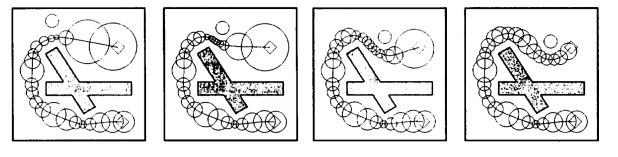
\includegraphics[height=2.5cm]{Figures/eband.png}
	\end{figure}
\end{frame}

%%%%%%%%%%%%%%%%%%%%%%%%%%%%%%%%%%%%%%%%%%%%%%%%%%%%%%%%%%%%%%%%%%%%%%%%%%%%%%%%%%%%%%%%%%%%%%
\begin{frame}{DPM (3/3): Μετατροπή Ελαστικής Ζώνης σε Ζώνη Reeds-Shepp}
\textbf{Μονοπάτι Reeds-Shepp}: βέλτιστο μονοπάτι για ένα αυτοκίνητο που κινείται και μπρος και πίσω
	\begin{itemize}
		\item 48 τύποι μονοπατιών Reeds-Shepp βάσει των λέξεων:
	\end{itemize}
	\vspace{-0.4cm}
	\begin{align*}
		\{C|C|C,\;CC|C,\;C|CC,\;CSC,\;CC_{\beta}|C_{\beta}C,\;	C|C_{\beta}C_{\beta}|C,\;\nonumber\\C|C_{\frac{\pi}{2}}SC,\;CSC_{\frac{\pi}{2}}|C,\;C|C_{\frac{\pi}{2}}SC_{\frac{\pi}2}|C\},\;\;\; C \in \{R,L\}
	\end{align*}

	\vspace{-0.5cm}	
	\begin{figure}
		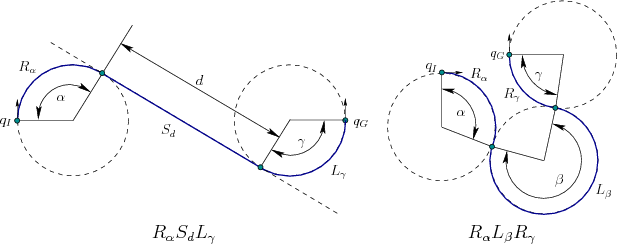
\includegraphics[height=2.5cm]{Figures/reeds_shepp_paths.png}
	\end{figure}

	\vspace{-0.2cm}	
	\begin{itemize}
		\item Ζώνη Reeds-Shepp $\rightarrow$ ακολουθία μονοπατιών Reeds-Shepp
	\end{itemize}
	
	\vspace{-0.5cm}
	\begin{figure}
		\captionsetup[subfigure]{labelformat=empty}
		\subfloat[Ολικό Μονοπάτι]{\frame{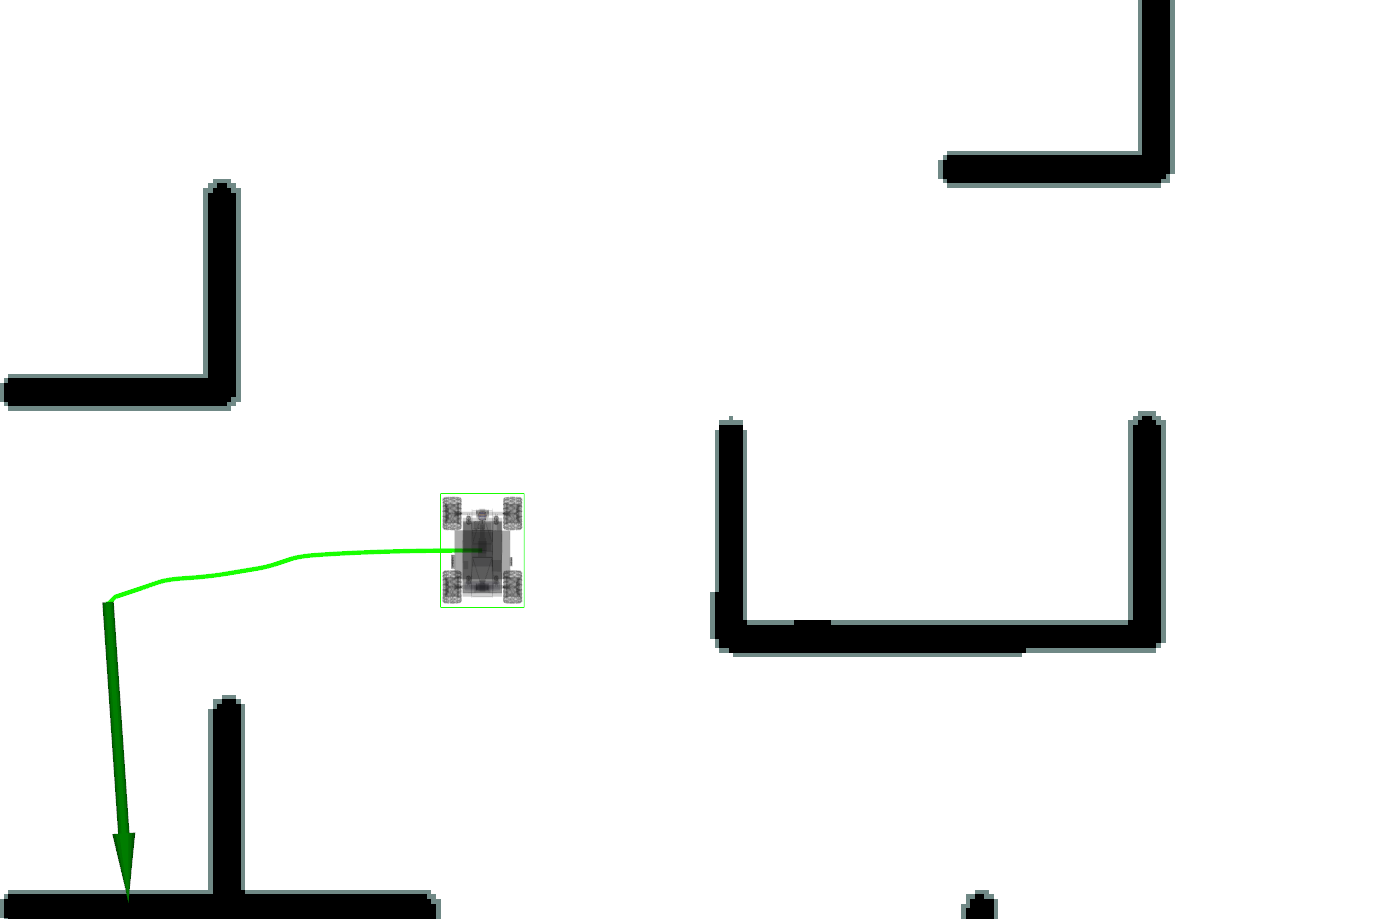
\includegraphics[height=1.5cm]{Figures/rsband_global_3.png}}} \hspace{0.5cm}
		\subfloat[Ελαστική Ζώνη]{\frame{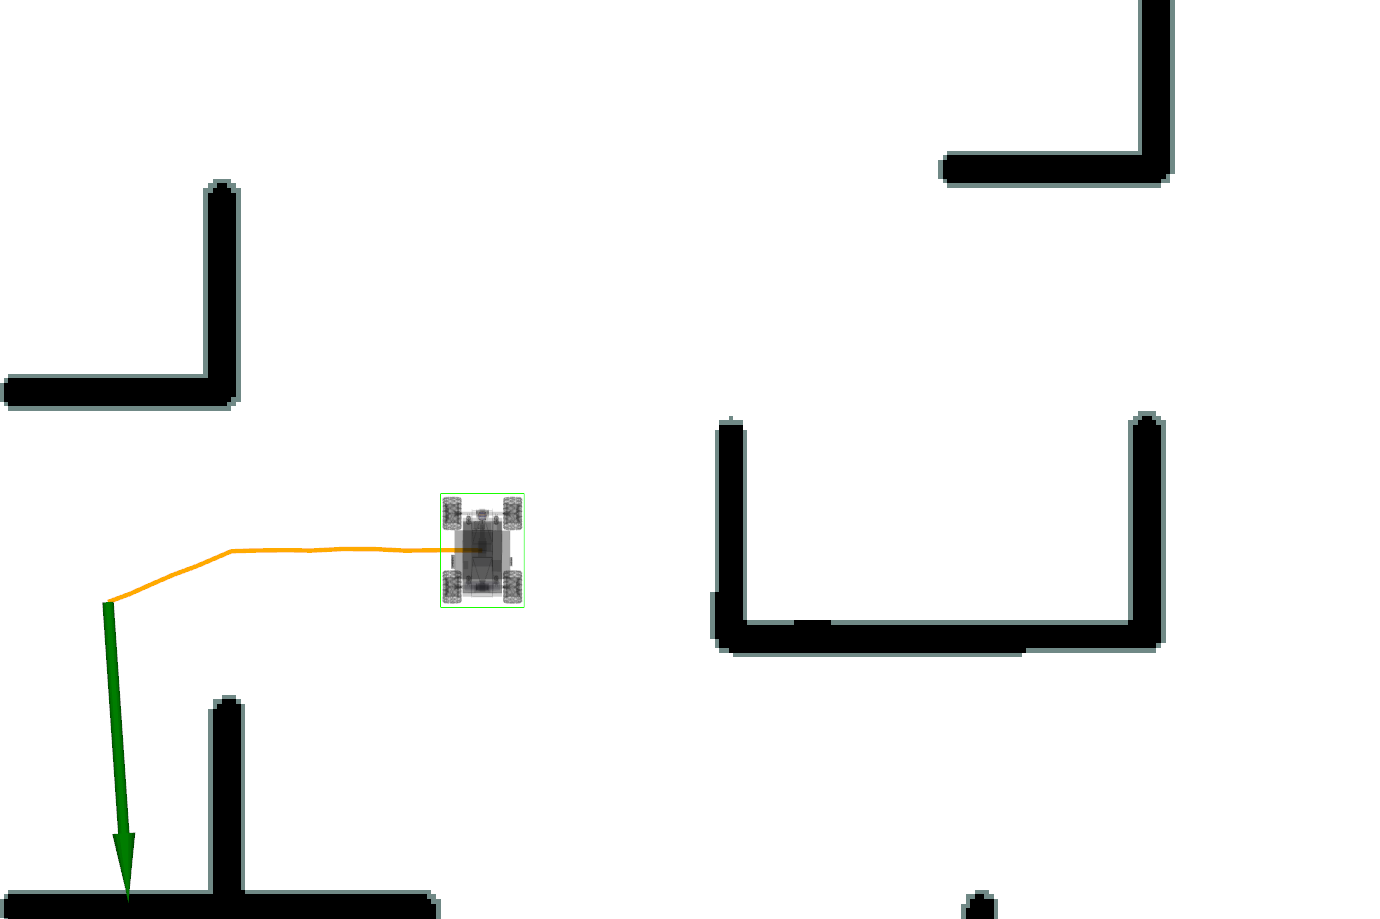
\includegraphics[height=1.5cm]{Figures/rsband_eband_3.png}}} \hspace{0.5cm}
		\subfloat[Ζώνη Reeds-Shepp]{\frame{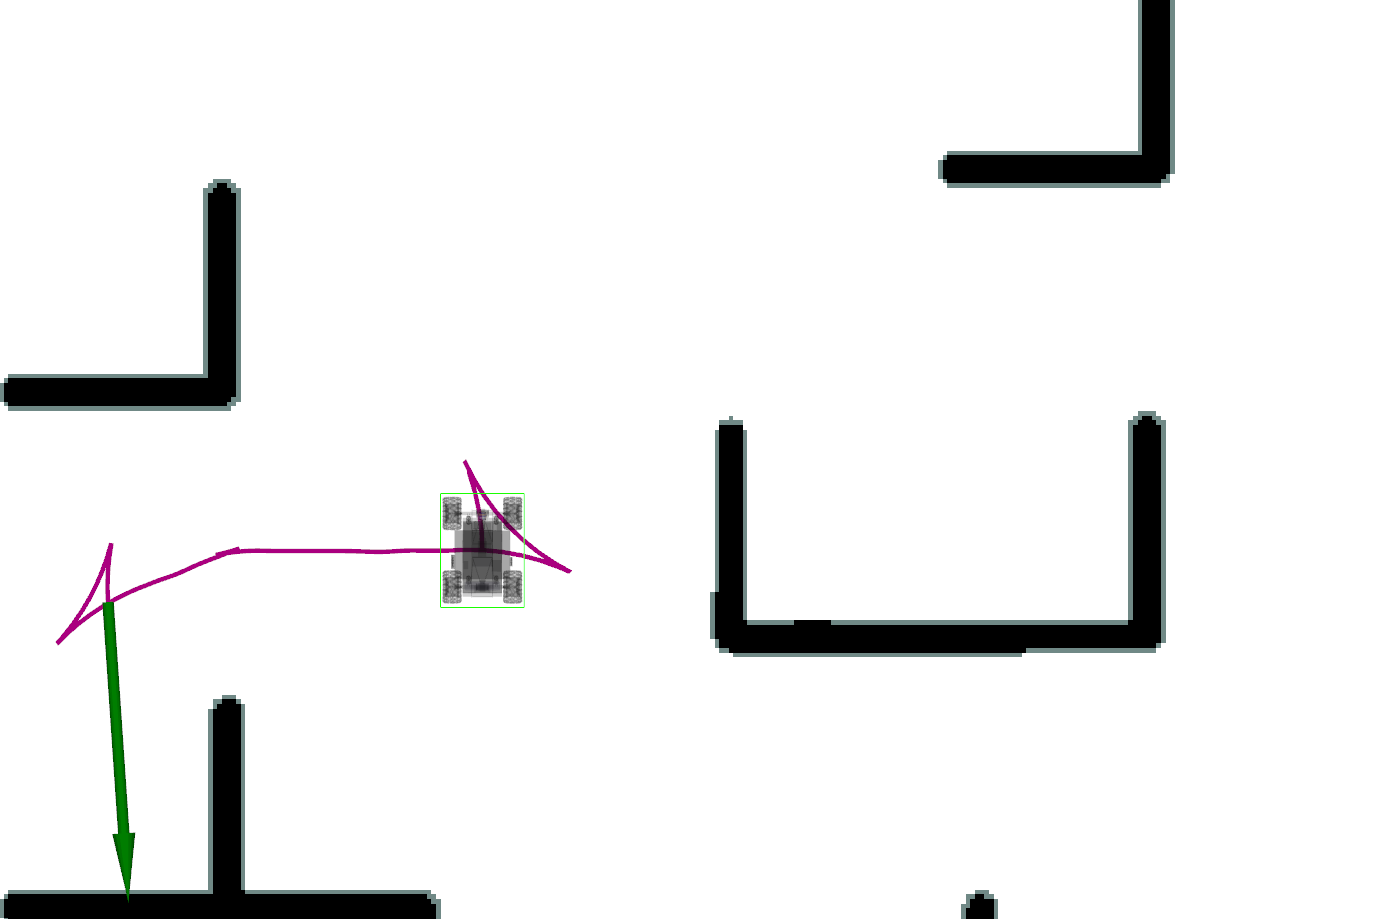
\includegraphics[height=1.5cm]{Figures/rsband_rsband_3.png}}}
	\end{figure}
\end{frame}

%%%%%%%%%%%%%%%%%%%%%%%%%%%%%%%%%%%%%%%%%%%%%%%%%%%%%%%%%%%%%%%%%%%%%%%%%%%%%%%%%%%%%%%%%%%%%%
\begin{frame}{DPR: SBPL Lattice Planner}
	\begin{itemize}
		\item Δικτύωμα Καταστάσεων όπου $s=(x,y,\theta,\upsilon)$\\$\rightarrow$ διακριτοποίηση χώρου καταστάσεων + συνδέσεις καταστάσεων
		\item Χώρος Κινήσεων: κινηματικά εφικτές κινήσεις
		\item Κατασκευή Μονοπατιού $\rightarrow$ αναζήτηση σε γράφο $\rightarrow$ ARA* ή AD*
	\end{itemize}
	\begin{figure}
		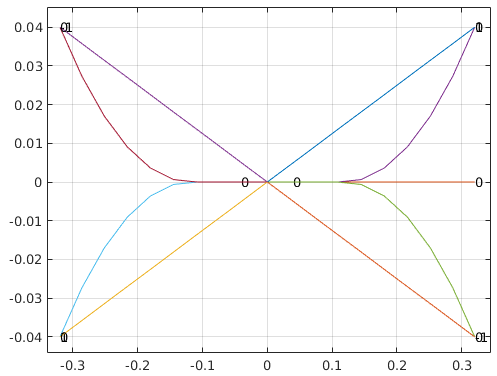
\includegraphics[height=3.0cm]{Figures/motion_primitives.png}
		\hspace{0.2cm}
		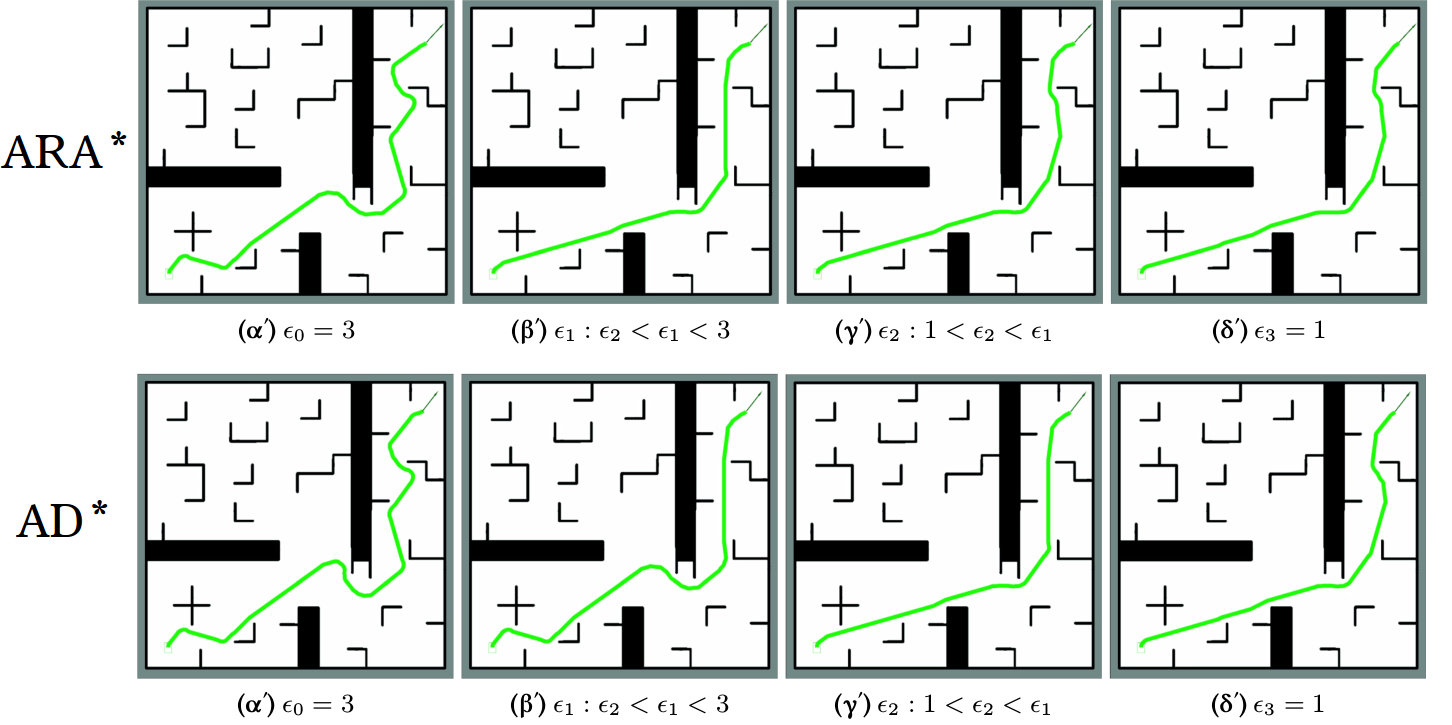
\includegraphics[height=3.0cm]{Figures/arastar_adstar.png}
	\end{figure}
\end{frame}

%%%%%%%%%%%%%%%%%%%%%%%%%%%%%%%%%%%%%%%%%%%%%%%%%%%%%%%%%%%%%%%%%%%%%%%%%%%%%%%%%%%%%%%%%%%%%%
%\begin{frame}{DPR (2/2): ARA* και AD*}
%	ARA*: Anytime Repairing A*\\
%	AD*: Anytime Dynamic A*
%	
%	\begin{itemize}
%		\item A* σε Μεγάλο πρόβλημα $\rightarrow$ παραβίαση χρονικών περιορισμών
%		\item Λύση: παραλλαγές του A* $\rightarrow$ ARA*, AD*
%		\item Αρχική μη βέλτιστη λύση και συνεχής βελτίωση
%		\item $\rightarrow$ $f(n) = g(n) + \epsilon \cdot h(n)$, $\epsilon \geq 1$
%		\item Επαναχρησιμοποίηση πληροφορίας από προηγούμενες αναζητήσεις
%		\item AD*: ARA* + D*/D* Lite $\rightarrow$ προσαρμογή σε δυναμικά εμπόδια
%	\end{itemize}
%	\begin{figure}
%		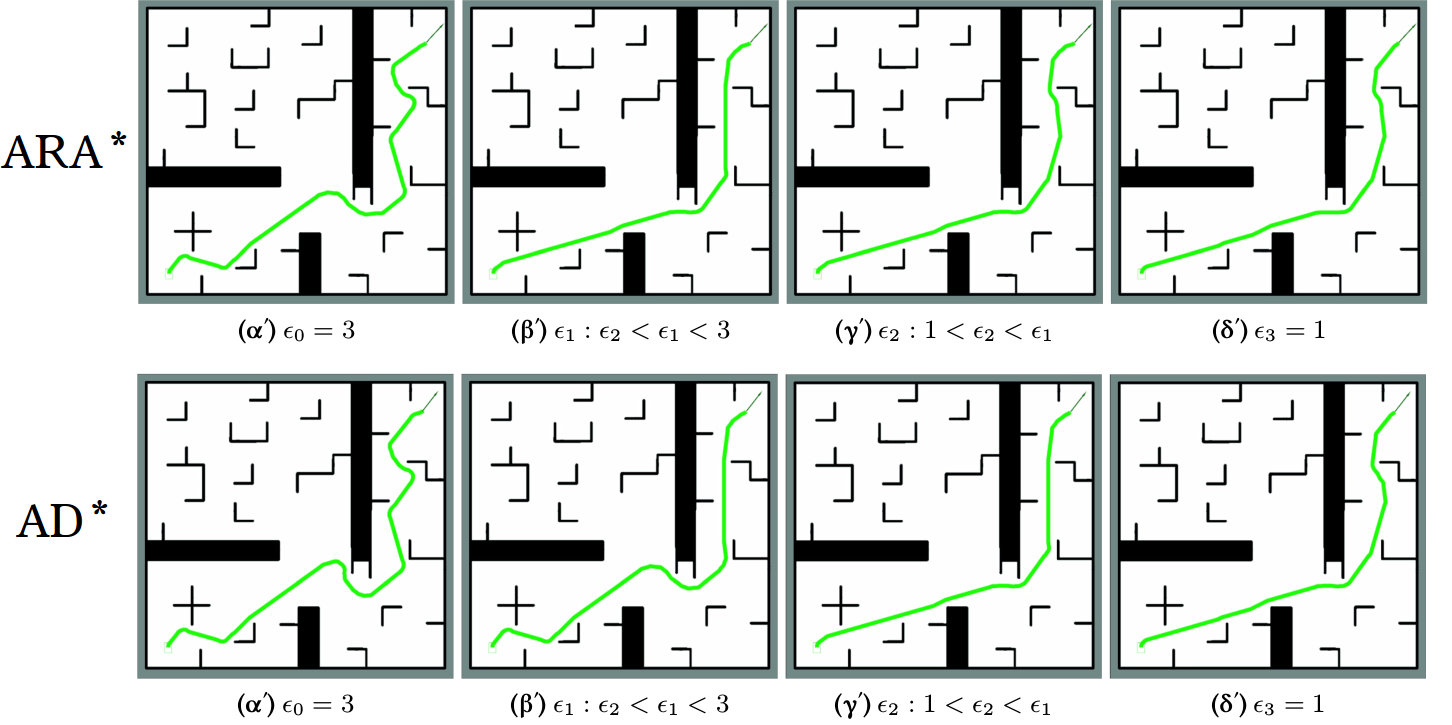
\includegraphics[height=4cm]{Figures/arastar_adstar.png}
%	\end{figure}
%\end{frame}

%%%%%%%%%%%%%%%%%%%%%%%%%%%%%%%%%%%%%%%%%%%%%%%%%%%%%%%%%%%%%%%%%%%%%%%%%%%%%%%%%%%%%%%%%%%%%%
\begin{frame}{Ασαφής Ελεγκτής Διάσχισης Μονοπατιού (1/2)}
	\begin{figure}
		\subfloat{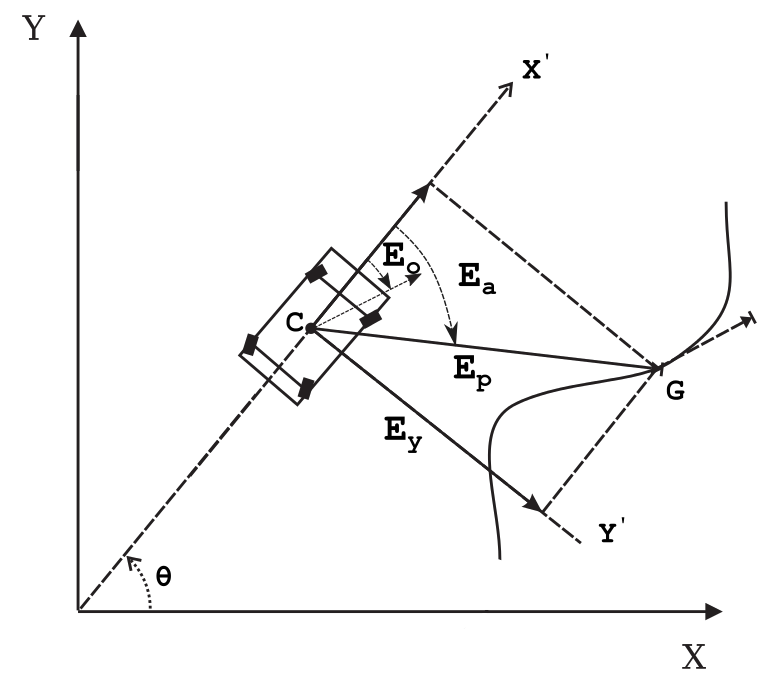
\includegraphics[height=4cm]{Figures/ptc_errors.png}}
		\hspace{1cm}
		\subfloat{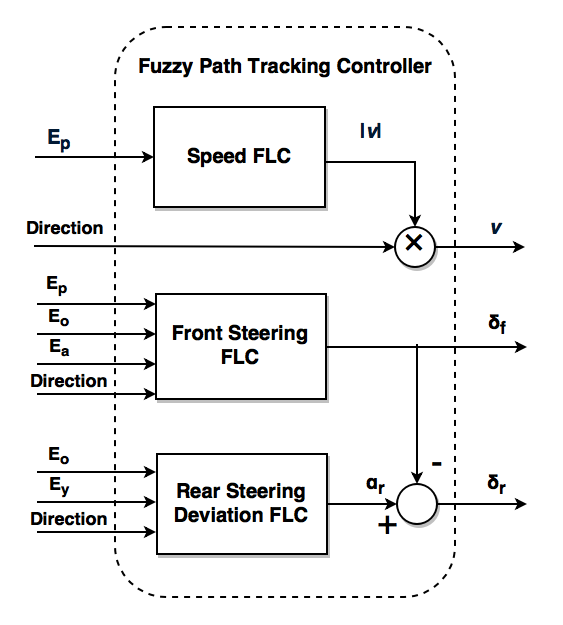
\includegraphics[height=4cm]{Figures/fuzzy_ptc_inside.png}}
	\end{figure}
	
	\begin{itemize}
		\item $\upsilon:$ ανάλογη της απόστασης $E_p$ από τον τρέχον στόχο
		\item $\delta_f:$ διόρθωση $E_\alpha$ μακρυά από τον στόχο και διόρθωση $E_o$ κοντά
		\item $\alpha_r:$ διόρθωση πλευρικής απόκλισης $E_y$ εάν $E_o$, $E_y$ μικρά
		\item Αντίστοιχη συμπεριφορά για κάθε φορά κίνησης ($Direction$)
	\end{itemize}
\end{frame}

%%%%%%%%%%%%%%%%%%%%%%%%%%%%%%%%%%%%%%%%%%%%%%%%%%%%%%%%%%%%%%%%%%%%%%%%%%%%%%%%%%%%%%%%%%%%%%
\begin{frame}{Ασαφής Ελεγκτής Διάσχισης Μονοπατιού (2/2)}
	\hspace{-0.5cm}
	\begin{minipage}{0.75\textwidth}
		\begin{figure}
			\centering
			\visible<1-3>{			
			\subfloat{
\includegraphics[height=2.5cm]{Figures/eo_ea_mf.png}}\\
			\subfloat{
\includegraphics[height=2.5cm]{Figures/ep_mf.png}}
			\subfloat{
\includegraphics[height=2.5cm]{Figures/ey_mf.png}}
			\subfloat{
\includegraphics[height=2.5cm]{Figures/direction_mf.png}}}\\
			\visible<2-3>{
			\subfloat{
\includegraphics[height=2.5cm]{Figures/speed_mf.png}}
			\subfloat{
\includegraphics[height=2.5cm]{Figures/df_dr_mf.png}}}
		\end{figure}
	\end{minipage}%
	\visible<3>{
	\begin{minipage}{0.24\textwidth}
		\begin{figure}
			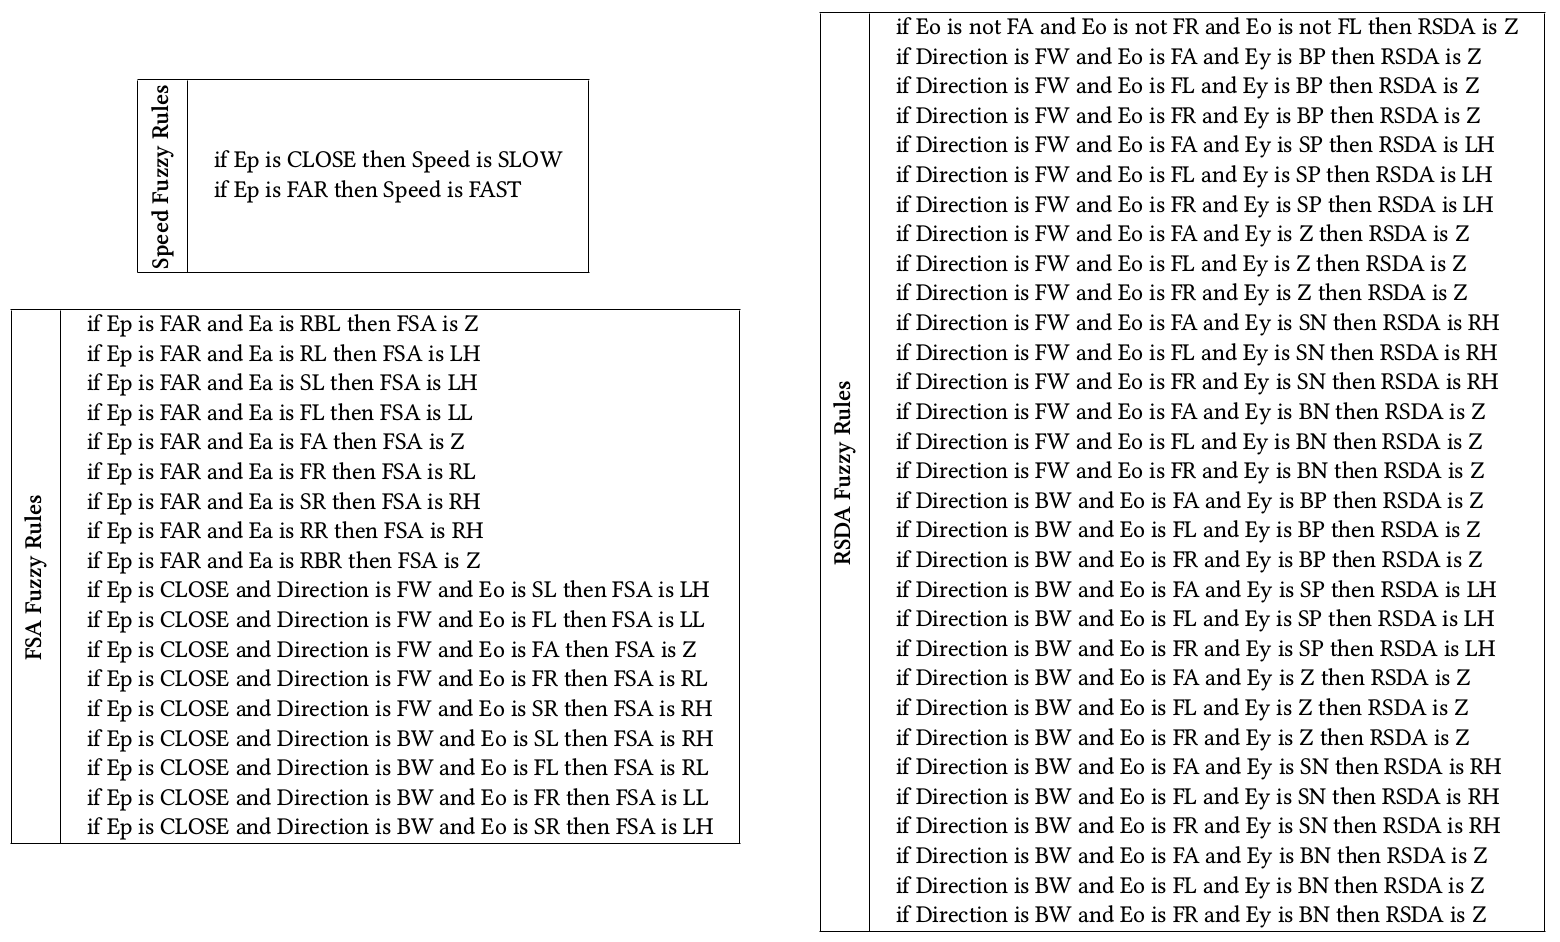
\includegraphics[height=8cm]{Figures/fuzzy_rules2.png}
		\end{figure}
	\end{minipage}}
\end{frame}

%%%%%%%%%%%%%%%%%%%%%%%%%%%%%%%%%%%%%%%%%%%%%%%%%%%%%%%%%%%%%%%%%%%%%%%%%%%%%%%%%%%%%%%%%%%%%%
\begin{frame}{Εξερεύνηση}
	\begin{itemize}
		\item Επιλογή στόχων
		\item Μέτωπο Εξερεύνησης $\rightarrow$ σύνορο
		\item Συνάρτηση κόστους $\rightarrow$ Κριτήρια επιλογής
		\begin{itemize}
			\item Μέγεθος μετώπου
			\item Μήκος μονοπατιού
			\item Γωνιακή απόκλιση
			\item Συχνότητα επιλογής
		\end{itemize}
	\end{itemize}
	\begin{figure}
		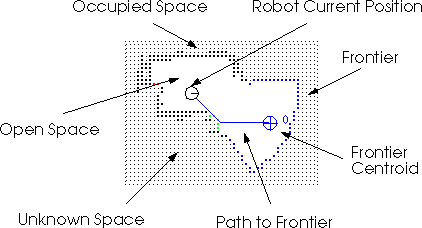
\includegraphics[width=0.7\linewidth]{Figures/frontier_exploration.png}
	\end{figure}
\end{frame}

%%%%%%%%%%%%%%%%%%%%%%%%%%%%%%%%%%%%%%%%%%%%%%%%%%%%%%%%%%%%%%%%%%%%%%%%%%%%%%%%%%%%%%%%%%%%%%
%%%%%%%%%%%%%%%%%%%%%%%%%%%%%%%%%%%%%%%%%%%%%%%%%%%%%%%%%%%%%%%%%%%%%%%%%%%%%%%%%%%%%%%%%%%%%%
\section{Εργαλεία και Αρχιτεκτονική Συστήματος}

%%%%%%%%%%%%%%%%%%%%%%%%%%%%%%%%%%%%%%%%%%%%%%%%%%%%%%%%%%%%%%%%%%%%%%%%%%%%%%%%%%%%%%%%%%%%%%
\begin{frame}{Εργαλεία}
	\begin{figure}
		
\includegraphics[width=0.4\linewidth]{Figures/ros.png}\\[0.5cm]
		\begin{tikzpicture}
			\pause
	   		\node (stdr_simulator) {{\includegraphics[height=3cm]{stdr_simulator.png}}};
		   \pause
		   \node (gazebo_simulator) at (stdr_simulator.south) [yshift=-0.9cm] [xshift=0cm] {{\includegraphics[height=3cm]{gazebo_simulator.png}}};
		\end{tikzpicture}
	\end{figure}
\end{frame}

%%%%%%%%%%%%%%%%%%%%%%%%%%%%%%%%%%%%%%%%%%%%%%%%%%%%%%%%%%%%%%%%%%%%%%%%%%%%%%%%%%%%%%%%%%%%%%
\begin{frame}{Διάγραμμα Τμημάτων Λογισμικού}
	\begin{figure}
		\includegraphics[width=\linewidth]{component_diagram.png}
	\end{figure}
\end{frame}

%%%%%%%%%%%%%%%%%%%%%%%%%%%%%%%%%%%%%%%%%%%%%%%%%%%%%%%%%%%%%%%%%%%%%%%%%%%%%%%%%%%%%%%%%%%%%%
%%%%%%%%%%%%%%%%%%%%%%%%%%%%%%%%%%%%%%%%%%%%%%%%%%%%%%%%%%%%%%%%%%%%%%%%%%%%%%%%%%%%%%%%%%%%%%
\section{Πειράματα}

\begin{frame}{Πειράματα Κινηματικού Μοντέλου}
	\visible<1-3>{	
	\begin{figure}
			\centering
			\subfloat{\frame{\includegraphics[height=2.7cm]{Figures/simple_room.png}}}
			\hspace{0.6cm}
			\subfloat{\frame{\includegraphics[height=2.7cm]{Figures/pandora_arena.png}}}
	\end{figure}}
	\vspace{-0.8cm}
	\visible<2-3>{	
	\begin{figure}
			\centering
			\subfloat{{\includegraphics[height=2.2cm]{Figures/counter_steering_experiment.png}}}
			\hspace{1.2cm}
			\subfloat{\frame{\includegraphics[height=2.2cm]{Figures/counter_steering_experiment_real.png}}}
			\hspace{0.8cm}
		\subfloat{{\includegraphics[height=2.2cm]{Figures/counter_steering_exp_plot.png}}}
	\end{figure}}
	\vspace{-0.8cm}
	\visible<3>{	
	\begin{figure}
		\centering
		\subfloat{{\includegraphics[height=2.2cm]{Figures/crab_steering_experiment.png}}}
		\hspace{1.2cm}
		\subfloat{\frame{\includegraphics[height=2.2cm]{Figures/crab_steering_experiment_real.png}}}
		\hspace{0.8cm}
		\subfloat{{\includegraphics[height=2.2cm]{Figures/crab_steering_exp_plot.png}}}
	\end{figure}	}
\end{frame}

%%%%%%%%%%%%%%%%%%%%%%%%%%%%%%%%%%%%%%%%%%%%%%%%%%%%%%%%%%%%%%%%%%%%%%%%%%%%%%%%%%%%%%%%%%%%%%
\begin{frame}{Πειράματα Χαρτογράφησης}
	\visible<1-3>{\begin{minipage}{0.3\textwidth}
		\begin{figure}
			\captionsetup[subfigure]{labelformat=empty}
			\subfloat[]{\includegraphics[height=2cm]{Figures/stdr_robocup_ground_truth.png}}\\
			\subfloat[]{\includegraphics[height=2cm]{Figures/robocup_2013_arena.png}}\\
			\subfloat[]{\frame{\includegraphics[height=2cm]{Figures/csal.jpg}}}
		\end{figure}
	\end{minipage}}
	\hspace{0.4cm}
	\visible<2-3>{
	\begin{minipage}{0.3\textwidth}
		\begin{figure}
			\captionsetup[subfigure]{labelformat=empty}
			\vspace{0.2cm}
			\subfloat[]{\includegraphics[height=2cm]{Figures/stdr_robocup_crsm.png}}\\
			\subfloat[]{\includegraphics[height=2cm]{Figures/robocup_arena_crsm_map.png}}\\
			\vspace{-0.3cm}
			\subfloat[]{\frame{\includegraphics[width=2.5cm]{Figures/csal_crsm_map.png}}}
		\end{figure}
	\end{minipage}}
	\hspace{0.2cm}
	\visible<3>{
	\begin{minipage}{0.3\textwidth}
		\begin{figure}
			\centering
			\vspace{0.2cm}
			\captionsetup[subfigure]{labelformat=empty}
			\subfloat[]{\includegraphics[height=2cm]{Figures/stdr_robocup_gmapping.png}}\\
			\subfloat[]{\includegraphics[height=2cm]{Figures/robocup_arena_gmapping_map.png}}\\
			\vspace{-0.3cm}
			\subfloat[]{\frame{\includegraphics[width=2.5cm]{Figures/csal_gmapping_map.png}}}
		\end{figure}
	\end{minipage}}
\end{frame}

%%%%%%%%%%%%%%%%%%%%%%%%%%%%%%%%%%%%%%%%%%%%%%%%%%%%%%%%%%%%%%%%%%%%%%%%%%%%%%%%%%%%%%%%%%%%%%
\begin{frame}{Πειράματα Κατασκευής Ολικού Μονοπατιού}
	\vspace{-0.4cm}
	\begin{table}
      \begin{tabular}{ c c }
			Dijkstra & \raisebox{-0.35\height}{\subfloat{\includegraphics[height=1.5cm]{Figures/dijkstra_exp.png}}}\\[-0.2cm]
			A* & \raisebox{-0.35\height}{\subfloat{\includegraphics[height=1.5cm]{Figures/astar_exp.png}}}\\[-0.2cm]
			ARA* & \raisebox{-0.35\height}{\subfloat{\includegraphics[height=1.5cm]{Figures/arastar_exp.png}}}\\[-0.2cm]
			AD* &	\raisebox{-0.35\height}{\subfloat{\includegraphics[height=1.5cm]{Figures/adstar_exp.png}}}
		\end{tabular}
	\end{table}

	\vspace{-0.3cm}
	\begin{table}
		\hspace{1.05cm}
		\resizebox{0.63\textwidth}{!}{
			\begin{tabular}{|c|cc|cc|cc|cc|}
				\cline{2-9}
				\multicolumn{1}{l|}{} & \multicolumn{2}{c|}{\textbf{Dijkstra}} & \multicolumn{2}{c|}{\textbf{A*}} & \multicolumn{2}{c|}{\textbf{ARA*}} & \multicolumn{2}{c|}{\textbf{AD*}} \\ 
				\cline{2-9}
				\multicolumn{1}{l|}{\multirow{-2}{*}{}} & \multicolumn{1}{c}{\textbf{$T[s]$}} & \multicolumn{1}{c|}{\textbf{$s[m]$}} & \multicolumn{1}{c}{\textbf{$T[s]$}} & \multicolumn{1}{c|}{\textbf{$s[m]$}} & \multicolumn{1}{c}{\textbf{$s_{init}[m]$}} & \multicolumn{1}{c|}{\textbf{$s_{final}[m]$}} & \multicolumn{1}{c}{\textbf{$s_{init}[m]$}} & {\textbf{$s_{final}[m]$}} \\ \hline
				\textbf{$p_1$} & 0.035 & 6.02 & 0.027 & 6.02 & 6.68 & 5.91 & 7.45 & 5.92\\
				\textbf{$p_2$} & 0.060 & 11.78 & 0.060 & 11.78 & 13.56 & 11.554 & 12.62 & 11.25\\ 
				\textbf{$p_3$} & 0.110 & 19.34 & 0.090 & 19.34 & 19.85 & 18.73 & 23.26 & 18.66\\
				\textbf{$p_4$} & 0.110 & 17.69 & 0.110 & 17.77 & 21.36 & 17.25 & 20.42 & 17.57\\ 
				\hline
			\end{tabular}}
		\end{table}
\end{frame}

%%%%%%%%%%%%%%%%%%%%%%%%%%%%%%%%%%%%%%%%%%%%%%%%%%%%%%%%%%%%%%%%%%%%%%%%%%%%%%%%%%%%%%%%%%%%%%
\begin{frame}{Πειράματα Δυναμικής Παραμόρφωσης Μονοπατιού}
	\begin{figure}
%		\includegraphics<1>[height=8cm]{Figures/rsband_free_space.png}
		\includegraphics<1>[height=8cm]{Figures/rsband_exp.png}
	\end{figure}		
\end{frame}

%%%%%%%%%%%%%%%%%%%%%%%%%%%%%%%%%%%%%%%%%%%%%%%%%%%%%%%%%%%%%%%%%%%%%%%%%%%%%%%%%%%%%%%%%%%%%%
\begin{frame}{Πειράματα Διάσχισης Μονοπατιού}
	\visible<1-3>{
	\begin{minipage}{0.5\textwidth}
		\begin{figure}
			\subfloat{\includegraphics[width=0.5\textwidth]{Figures/zic_zac_room_no_ramps.png}}
			\subfloat{\includegraphics[width=0.5\textwidth]{Figures/zic_zac_room_no_ramps_path_and_traj.png}}
		\end{figure}	
	\end{minipage}%
	\begin{minipage}{0.5\textwidth}
		\includegraphics[width=\textwidth]{Figures/fsa_rsa_1.png}
	\end{minipage}\\[0.5cm]}

	\visible<2-3>{
	\begin{minipage}{0.5\textwidth}
		\begin{figure}
			\subfloat{\includegraphics[width=0.5\textwidth]{Figures/zic_zac_room.png}}
			\subfloat{\includegraphics[width=0.5\textwidth]{Figures/zic_zac_room_path_and_traj.png}}
		\end{figure}	
	\end{minipage}%
	\begin{minipage}{0.5\textwidth}
		\includegraphics[width=\textwidth]{Figures/fsa_rsa_2.png}
	\end{minipage}\\[0.5cm]}

	\visible<3>{
	\begin{minipage}{0.5\textwidth}
		\begin{figure}				
			\subfloat{\includegraphics[width=\textwidth]{Figures/slope_room.png}}\\[-0.1cm]
			\subfloat{\includegraphics[width=\textwidth]{Figures/slope_room_path_and_traj.png}}
		\end{figure}
	\end{minipage}%
	\begin{minipage}{0.5\textwidth}
		\includegraphics[width=\textwidth]{Figures/fsa_rsa_3.png}
	\end{minipage}}
\end{frame}

%%%%%%%%%%%%%%%%%%%%%%%%%%%%%%%%%%%%%%%%%%%%%%%%%%%%%%%%%%%%%%%%%%%%%%%%%%%%%%%%%%%%%%%%%%%%%%
\begin{frame}{Πειράματα Εξερεύνησης Πραγματικού Περιβάλλοντος}
	\begin{figure}
      \captionsetup[subfigure]{labelformat=empty,position=top}
		\subfloat[DPM]{\frame{\includegraphics[height=4.5cm]{Figures/exploration_dpm.png}}}
		\hspace{0.05\linewidth}
		\subfloat[DPR]{\frame{\includegraphics[height=4.5cm]{Figures/exploration_dpr.png}}}
	\end{figure}	

	\begin{table}[!ht]
		\centering
		\resizebox{0.3\textwidth}{!}{
		\begin{tabular}{|c|c|c|}	\hline
			 & $\mathbf{T_E[s]}$ & $\mathbf{S_E[m]}$\\ \hline
			\textbf{DPM} & $486$ & $114.89$\\ \hline
			\textbf{DPR} & $698$ & $93.38$\\ \hline
		\end{tabular}}
	\end{table}
\end{frame}

%%%%%%%%%%%%%%%%%%%%%%%%%%%%%%%%%%%%%%%%%%%%%%%%%%%%%%%%%%%%%%%%%%%%%%%%%%%%%%%%%%%%%%%%%%%%%%
%%%%%%%%%%%%%%%%%%%%%%%%%%%%%%%%%%%%%%%%%%%%%%%%%%%%%%%%%%%%%%%%%%%%%%%%%%%%%%%%%%%%%%%%%%%%%%
\section{Συμπεράσματα και Μελλοντικές Επεκτάσεις}

%%%%%%%%%%%%%%%%%%%%%%%%%%%%%%%%%%%%%%%%%%%%%%%%%%%%%%%%%%%%%%%%%%%%%%%%%%%%%%%%%%%%%%%%%%%%%%
\begin{frame}{Συμπεράσματα}
	\begin{itemize}
		\item Μικρά σφάλματα κινηματικού μοντέλου
		\item Ατέλειες χαρτογράφησης, αλλά επαρκής αναπαράσταση
		\item DPM: υψηλή συχνότητα, αλλά αστάθεια υπό περιπτώσεις
		\item DPR: ευσταθής συμπεριφορά, αλλά χαμηλή συχνότητα
		\item Διάσχιση Μονοπατιού: επιτυχής αντιστάθμιση σφαλμάτων, αλλά κίνδυνος σύγκρουσης
	\end{itemize}
\end{frame}

%%%%%%%%%%%%%%%%%%%%%%%%%%%%%%%%%%%%%%%%%%%%%%%%%%%%%%%%%%%%%%%%%%%%%%%%%%%%%%%%%%%%%%%%%%%%%%
\begin{frame}{Μελλοντικές Επεκτάσεις}
	\begin{itemize}
		\item Βελτίωση	μηχανολογικής κατασκευής
		\item Επέκταση ρομποτικής αντίληψης
		\item Ενσωμάτωση αλγορίθμων ρομποτικής όρασης
		\item Αποδοτικότερος αλγόριθμος κατασκευής μονοπατιών Reeds-Shepp
		\item Διάσχιση μονοπατιού με εντοπισμό εμποδίων
	\end{itemize}
\end{frame}

%%%%%%%%%%%%%%%%%%%%%%%%%%%%%%%%%%%%%%%%%%%%%%%%%%%%%%%%%%%%%%%%%%%%%%%%%%%%%%%%%%%%%%%%%%%%%%
\begin{frame}{Ερωτήσεις}
	\begin{figure}
		\includegraphics[height=6cm]{Figures/question_mark.png}
	\end{figure}
\end{frame}

%%%%%%%%%%%%%%%%%%%%%%%%%%%%%%%%%%%%%%%%%%%%%%%%%%%%%%%%%%%%%%%%%%%%%%%%%%%%%%%%%%%%%%%%%%%%%%
\begin{frame}[allowframebreaks]{Βιβλιογραφία}
	\nocite{*}
	\printbibliography
\end{frame}

\end{document}
